\documentclass[11pt]{beamer}

%%%%%%%% tema e cor %%%%%%%%
\mode<presentation> {
    \usetheme{Boadilla}
    \usecolortheme{whale}
    \definecolor{UBCblue}{HTML}{32A041} % UBC Blue (primary)
    \usecolortheme[named=UBCblue]{structure}
}

\usepackage[brazil]{babel}
\usepackage[utf8]{inputenc}

\usepackage{graphicx} 
\usepackage{booktabs} 
\usepackage{caption}
\usepackage[most]{tcolorbox}
\usepackage{subcaption}
\usepackage{algorithmicx}
\usepackage[ruled]{algorithm}
\usepackage{algpseudocode}

\institute[IFMG] 
{
%================= logos no meio =====================
\vspace*{0.40cm}\\

\includegraphics[scale=0.35]{img/logo/Ifmg.png}
\vspace*{0.35cm}\\
Instituto Federal de Educação, Ciência e Tecnologia de Minas Gerais Campus \\
Formiga – IFMG \\
%\medskip
%\texttt{\{lods.eng,ronety\}@uea.edu.br} % emails
}
\date{14 de novembro de 2023}

\AtBeginSection[]
{
\begin{frame}
\frametitle{Conteúdo}
\tableofcontents[currentsection]
\end{frame}
}

%%%%%%%% titulo e subtitulo %%%%%%%%
\title[Trabalho de Conclusão de Curso]{Ferramenta de visão computacional para monitoramento do movimento de barra fixa voltado para testes de aptidão física } 

%%%%%%%% nome dos autores %%%%%%%%
\author[Fernandes, L. M.]{
Lucas Mateus Fernandes} 

\begin{document}
\begin{frame}
\titlepage 
\end{frame}

\begin{frame}
\frametitle{Conteúdo} 
\tableofcontents 
\end{frame}

%%%%%%%% slides %%%%%%%%
\section{Introdução} 
%%%%%%%%%%%%%%%%%%%%%%%%%%%%%%%%%%%%%%%%%%%%%%%%%%%%%%%%%%%%%%%%%%%%
%%
%%                     Introdução
%%
%%%%%%%%%%%%%%%%%%%%%%%%%%%%%%%%%%%%%%%%%%%%%%%%%%%%%%%%%%%%%%%%%%%%


\begin{frame}{Introdução}

    \begin{figure}[!ht]
        \centering % para centralizar a figur
          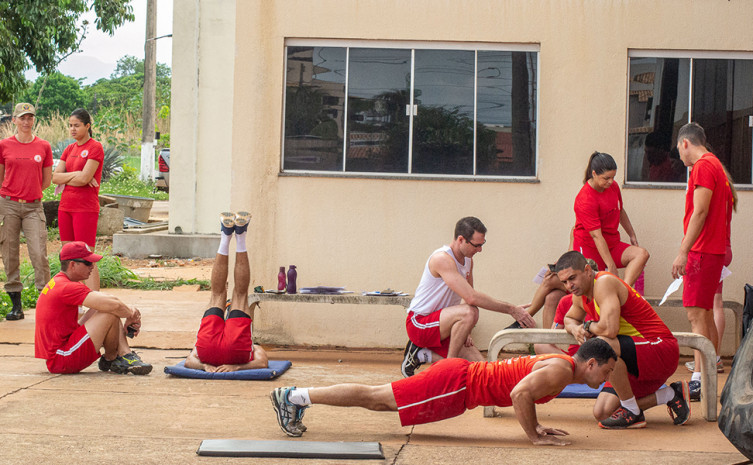
\includegraphics[scale=0.5]{img/intro/taf.jpeg}
         \caption{Teste de Aptidão Física - (TAF)}
    \end{figure}

\end{frame}


\begin{frame}{Introdução}

    \begin{figure}[!ht]
        \centering % para centralizar a figur
          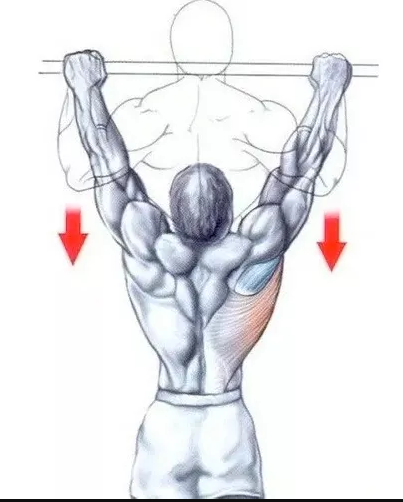
\includegraphics[scale=0.35]{img/intro/barra_fixa.png}
         \caption{Barra Fixa}
    \end{figure}

\end{frame}


%%%%%%%%%%%%%%%%%%%%%%%%%%%%%%%%%%%%%%%%%%%%%%%%%%%%%%%%%%%%%%%%%%%%
%%
%%                     Justificativa
%%
%%%%%%%%%%%%%%%%%%%%%%%%%%%%%%%%%%%%%%%%%%%%%%%%%%%%%%%%%%%%%%%%%%%%


\begin{frame}{Justificativa}
    \begin{block}{ Potencial para aumentar a confiabilidade e justiça do processo seletivo}
        \begin{itemize}
            \item  Minimiza os efeitos da fadiga de decisão dos avaliadores;
            \item  Minimiza a subjetividade na avaliação do exercício de barra fixa;
        \end{itemize}
    \end{block}
\end{frame}


\begin{frame}{Justificativa}
    \begin{block}{Contribuição para a evolução da maturidade da consciência corporal do indivíduo.}
        \begin{itemize}
            \item A percepção durante o exercício é essencial para o aprimoramento do movimento.
            \item Gera a tomada de consciência do corpo em relação ao movimento da barra fixa.
        \end{itemize}
    \end{block}
\end{frame}


\begin{frame}{Justificativa}
    \begin{block}{Contribuição para o treinamento no TAF}
        \begin{itemize}
            \item Fornece o feedback sobre a execução correta do movimento.
        \end{itemize}
    \end{block}
\end{frame}




%%%%%%%%%%%%%%%%%%%%%%%%%%%%%%%%%%%%%%%%%%%%%%%%%%%%%%%%%%%%%%%%%%%%
%%
%%                     Objetivos
%%
%%%%%%%%%%%%%%%%%%%%%%%%%%%%%%%%%%%%%%%%%%%%%%%%%%%%%%%%%%%%%%%%%%%%

\begin{frame}{Objetivos}
    \begin{block}{Objetivo Geral}
    Este trabalho tem como objetivo projetar e desenvolver uma ferramenta de visão computacional para análise do movimento de barra fixa associada ao TAF.
    \end{block}

\end{frame}



\begin{frame}{Objetivos}
   
    \begin{block}{Objetivos Específicos}
        \begin{itemize}
            \item Desenvolver uma ferramenta de visão computacional (em nível de prova de conceito) que analise o movimento de barra fixa.
                \begin{itemize}
                    \item Identificar a corretude do movimento de barra fixa.
                    \item Definir um procedimento para estabelecer a corretude do movimento de barra fixa, tendo como parâmetros alguns editais de concursos públicos da esfera militar
                    \item Analisar o movimento de barra fixa de modo a auxiliar na formação da consciência corporal do indivíduo por meio de feedback.
                \end{itemize}
            \item Usar a visão computacional para validar a corretude do movimento de barra fixa, tendo como parâmetros alguns editais de concursos públicos da esfera militar.
        \end{itemize}
    \end{block}

\end{frame}






\section{Fundamentação Teórica}
\begin{frame}{Transformada de Hough}
    \begin{itemize}
        \item A transformada de Hough é capaz de detectar grupos de pixels que pertencem a uma linha reta (mesmo que esteja quebrada ou com ruídos).
        
        \item Uma reta pode ser descrita como:  y = mx + b
        
        \item Pela parametrização $\rho = x \protect\ast \cos(\theta) + y \protect\ast \sin(\theta)$

        
        \item Onde o parâmetro $\rho$ é a mínima distância da reta a origem, centro do plano, e $\theta$ é o ângulo de inclinação da normal à reta, sendo a normal uma linha perpendicular a direção da reta
        
        \item Dois pontos \textbf{p} e \textbf{q} no plano da imagem definem uma reta \textbf{pq} e correspondem a dois senoides no plano de Hough, a intersecção dos dois senóides representa a reta \textbf{pq} que passa pelos dois pontos no plano da imagem
    \end{itemize}
\end{frame}

\section{Materiais e Métodos}
%%%%%%%%%%%%%%%%%%%%%%%%%%%%%%%%%%%%%%%%%%%%%%%%%%%%%%%%%%%%%%%%%%%%
%%
%%                     Materiais
%%
%%%%%%%%%%%%%%%%%%%%%%%%%%%%%%%%%%%%%%%%%%%%%%%%%%%%%%%%%%%%%%%%%%%%

    \begin{frame}{Materiais}
       \begin{figure}[!ht]
        \centering % para centralizar a figur
          %
          \begin{subfigure}[H]{0.3\textwidth}
            
\includegraphics[width=\textwidth]{img/logo/Python.png}
            \label{fig_op_ag}
          \end{subfigure}
          \hspace*{0.80cm}
          \begin{subfigure}[H]{0.2\textwidth}
            
\includegraphics[width=\textwidth]{img/logo/OpenCv.png}
            \label{fig_op_af}
          \end{subfigure}
          \hspace*{0.80cm}
          \begin{subfigure}[H]{0.3\textwidth}
            
\includegraphics[width=\textwidth]{img/logo/MediaPipe.png}
            \label{fig_op_af}
          \end{subfigure}
          \begin{subfigure}[H]{0.3\textwidth}
            
\includegraphics[width=\textwidth]{img/logo/Git.png}
          \end{subfigure}
          
      
    \end{figure}
\end{frame}


%%%%%%%%%%%%%%%%%%%%%%%%%%%%%%%%%%%%%%%%%%%%%%%%%%%%%%%%%%%%%%%%%%%%
%%
%%                     Método
%%
%%%%%%%%%%%%%%%%%%%%%%%%%%%%%%%%%%%%%%%%%%%%%%%%%%%%%%%%%%%%%%%%%%%%

\begin{frame}{Método}
    \begin{enumerate}
        \item Realização de revisão da literatura abordando o uso de visão computacional associado ao treinamento físico.
        \vspace*{0.80cm}
        \item Escolha das tecnologias.
        \vspace*{0.80cm}
        \item Criação de uma estrategia para deteção do movimento correto de barra fixa
        \vspace*{0.80cm}
        \item Desenvolvimento de uma Ferramenta computacional para detecção da execução correta da barra fixa.
    \end{enumerate}
\end{frame}


\begin{frame}{Método}
    \begin{figure}[!ht]
        \centering
        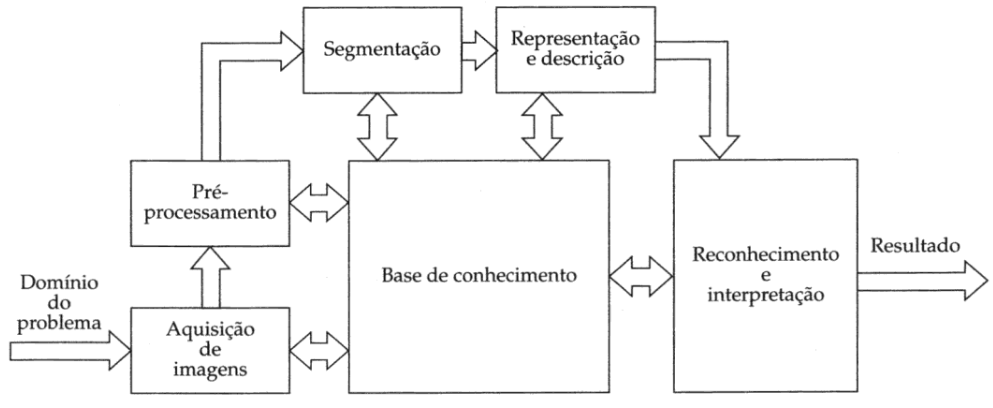
\includegraphics[scale=0.33]{img/metodos/processamentoImagem.png}
        \caption*{(GONZALEZ; WOODS, 2000)}
    \end{figure}
\end{frame}

\section{Projeto e Desenvolvimento}
%%%%%%%%%%%%%%%%%%%%%%%%%%%%%%%%%%%%%%%%%%%%%%%%%%%%%%%%%%%%%%%%%%%%
%%
%%                     AFD
%%
%%%%%%%%%%%%%%%%%%%%%%%%%%%%%%%%%%%%%%%%%%%%%%%%%%%%%%%%%%%%%%%%%%%%

\begin{frame}{Definição do movimento de barra fixa}
    \begin{itemize}
        \item A \textbf{barra} fixa é instalada a uma altura tal, que o avaliado, mantendo-se pendurado, com os cotovelos em extensão, não tenha contato dos pés com o solo;
        \item  A posição da \textbf{pegada} é pronada (dorso da mão voltado para o rosto) e a abertura das mãos corresponde à distância biacromial (largura dos ombros); 
        \item  Após assumir essa posição, o avaliado deverá elevar o corpo até que o \textbf{queixo ultrapasse o nível da barra}, após o que retornará à posição inicial; 
        \item  O movimento é \textbf{repetido} tantas vezes quanto possível, sem limite de tempo. 
    \end{itemize}
\end{frame}

\begin{frame}{Definição do movimento de barra fixa}
    \begin{itemize}
        \item  Os cotovelos deverão estar em \textbf{extensão} total para o início de flexão; 
        \item  É permitido \textbf{repouso} entre um movimento e outro, contudo, o avaliado não poderá tocar os pés no solo; 
        \item  \textbf{Não são permitidos} movimentos de quadris ou pernas e extensão da coluna cervical como formas de auxiliar na execução da prova. 
        \item  A não extensão total dos cotovelos antes do início de nova execução é considerado um \textbf{movimento incorreto}, o qual não será computado no desempenho do candidato. 
        \item  Somente é contado o número de movimentos completados corretamente.
    \end{itemize}
\end{frame}


\begin{frame}{Estratégia para detecção do movimento correto de barra fixa}

    \begin{figure}[!ht]
    \centering
    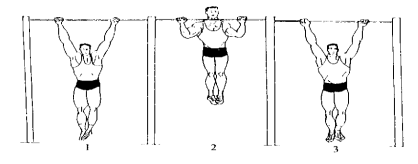
\includegraphics[scale=0.5]{img/desenvolvimento/barraFixa/barraFixa.jpg}
    \caption*{Fonte - (GOIÁS, 2017)}
    \end{figure}

    
    \begin{enumerate}
        \item  A primeira etapa engloba a posição inicial.

        \item  A segunda etapa engloba a fase de contração concêntrica, onde o indivíduo eleva seu corpo até que seu queixo ultrapasse o nível da barra.

        \item  A terceira etapa engloba a fase de contração excêntrica.
    \end{enumerate}
\end{frame}


\begin{frame}{Computação do movimento barra fixa}

    \begin{figure}[!ht]
    \centering
    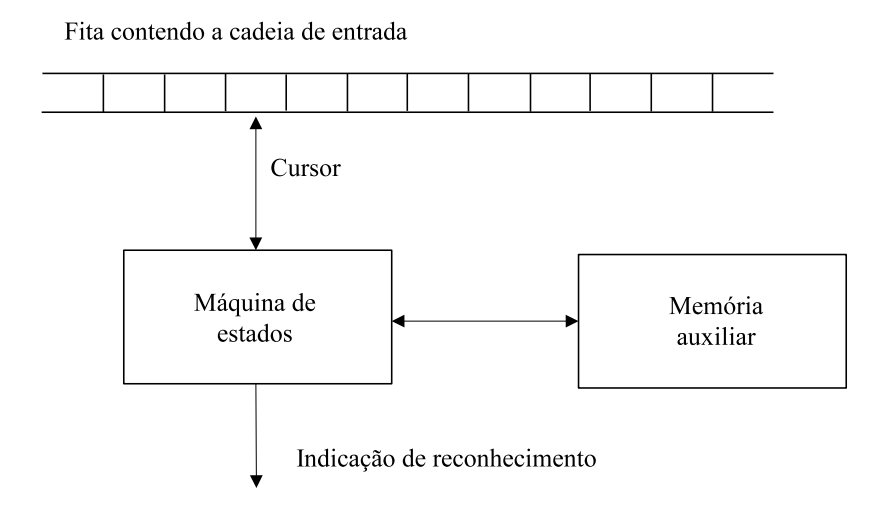
\includegraphics[scale=1.3]{img/desenvolvimento/estrategia/reconhecedor.png}
    \caption*{Fonte - (OLIVETE, 2020).}
    \end{figure}
    
\end{frame}


\begin{frame}{Composição do alfabeto}
    
    O AFD construído opera em relação a um alfabeto específico. Esse alfabeto é constituído por características extraídas de cada \textit{frame}. Cada símbolo do alfabeto é representado por uma 4-upla de características (A,B,C,D)
    
    \begin{itemize}
        \item[A] - Presença das mãos na barra.
        \item[B] - Ocorrência da extensão dos cotovelos.
        \item[C] - Ocorrência da ultrapassagem do queixo sobre a barra.
        \item[D] - Existência de movimento nos quadris.
    \end{itemize} 

\end{frame}



\begin{frame}{Alfabeto}
    \[
    \begin{aligned}
    \Sigma = \{ &(0, 0, 0, 0), (0, 0, 0, 1), (0, 0, 1, 0), (0, 0, 1, 1), \\
                &(0, 1, 0, 0), (0, 1, 0, 1), (0, 1, 1, 0), (0, 1, 1, 1), \\
                &(1, 0, 0, 0), (1, 0, 0, 1), (1, 0, 1, 0), (1, 0, 1, 1), \\
                &(1, 1, 0, 0), (1, 1, 0, 1), (1, 1, 1, 0), (1, 1, 1, 1) \}
    \end{aligned}
    \]
\end{frame}


\begin{frame}{Estados}
    O AFD desenvolvido consiste em um conjunto de sete estados:\\
    \vspace{0.8cm}
    $Q$ = \{Preparação, Início, Concêntrica, Meta, Excêntrica, Erro, Fim\}
     
\end{frame}



\begin{frame}{Diagrama de Estados}

    \begin{figure}[!ht]
    \centering
    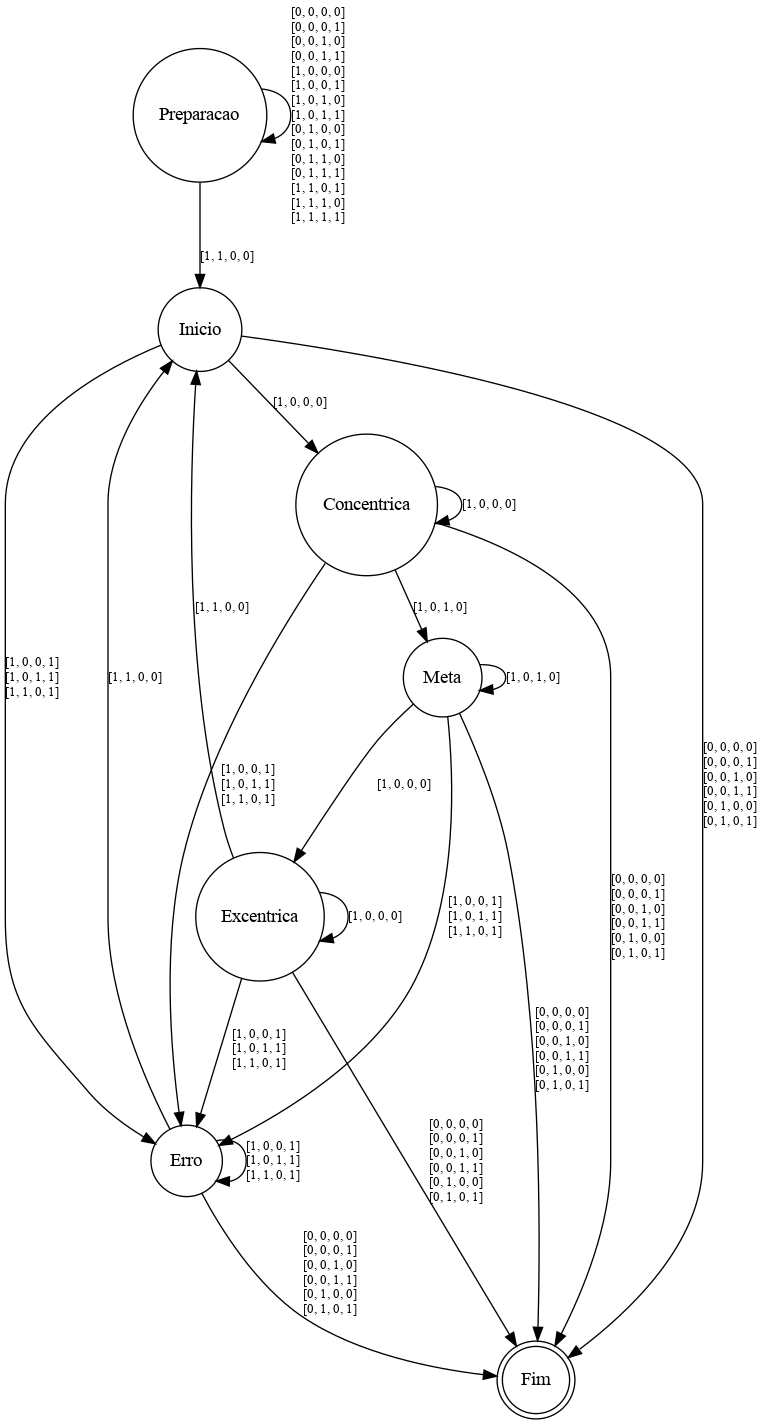
\includegraphics[scale=0.13]{img/desenvolvimento/estrategia/afd_barra.png}
    \caption*{Fonte - Proprio autor 2023.}
    \end{figure}
    
\end{frame}


%%%%%%%%%%%%%%%%%%%%%%%%%%%%%%%%%%%%%%%%%%%%%%%%%%%%%%%%%%%%%%%%%%%%
%%
%%                     Processos
%%
%%%%%%%%%%%%%%%%%%%%%%%%%%%%%%%%%%%%%%%%%%%%%%%%%%%%%%%%%%%%%%%%%%%%


\begin{frame}{Extração de informação frame a frame}
    \begin{itemize}
        \item  Detecção da barra 
        \item  Inclinação da barra
        \item  Reconhecimento de pose humana 
        \item  Mão na barra 
        \item  Braço esticado
        \item  Ultrapassagem do queixo a barra
        \item  Movimentação do quadril
    \end{itemize}
\end{frame}






%%%%%%%%%%%%%%%%%%%%%%%%%%%%%%%%%%%%%%%%%%%%%%%%%%%%%%%%%%%%%%%%%%%%
%%
%%                     Método
%%
%%%%%%%%%%%%%%%%%%%%%%%%%%%%%%%%%%%%%%%%%%%%%%%%%%%%%%%%%%%%%%%%%%%%
%%
%%                     Detecção da barra
%%
%%%%%%%%%%%%%%%%%%%%%%%%%%%%%%%%%%%%%%%%%%%%%%%%%%%%%%%%%%%%%%%%%%%%


\begin{frame}{Detecção da barra - Fluxograma}
    \begin{figure}[!ht]
    \centering
    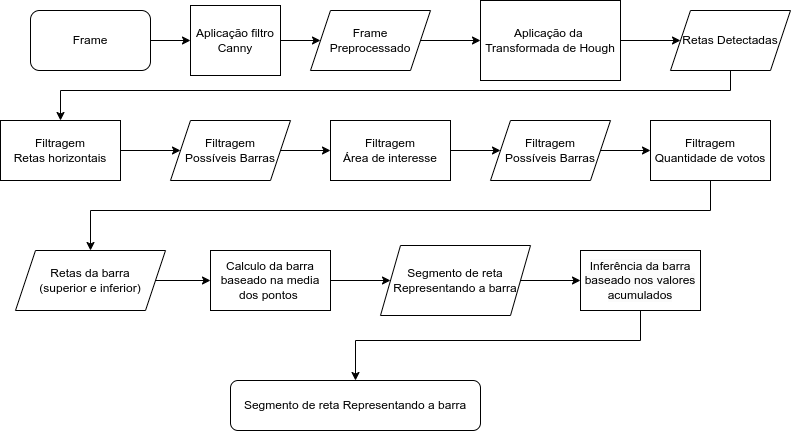
\includegraphics[scale=0.4]{img/desenvolvimento/detectaBarra/fluxograma.png}
    \caption*{Fonte - Próprio Autor.}
    \end{figure}
\end{frame}

\begin{frame}{Detecção da barra - Filtro de Canny.}
    \begin{itemize}
        \item  Redução de ruído         (Gaussiano - Blur)
        \item  Cálculo do Gradiente     (Sobel - detecção de contornos)
        \item  Supressão não máxima     (Filtro Passa Alta) 
        \item  Limite duplo             (minVal e maxVal)
        \item  Limite de histerese      (conectividade)
    \end{itemize}
\end{frame}

\begin{frame}{Detecção da barra - Aplicação do filtro de Canny.}
    \begin{figure}[!ht]
    \centering
    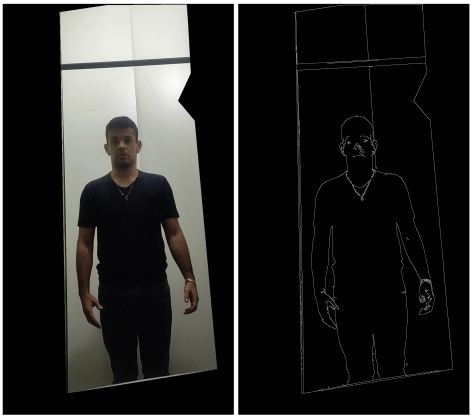
\includegraphics[scale=0.45]{img/desenvolvimento/detectaBarra/canny.png}
    \caption*{Fonte - Próprio Autor.}
    \end{figure}
\end{frame}



\begin{frame}{Detecção da barra - Segmentos de Retas.}
    \begin{figure}[!ht]
    \centering
    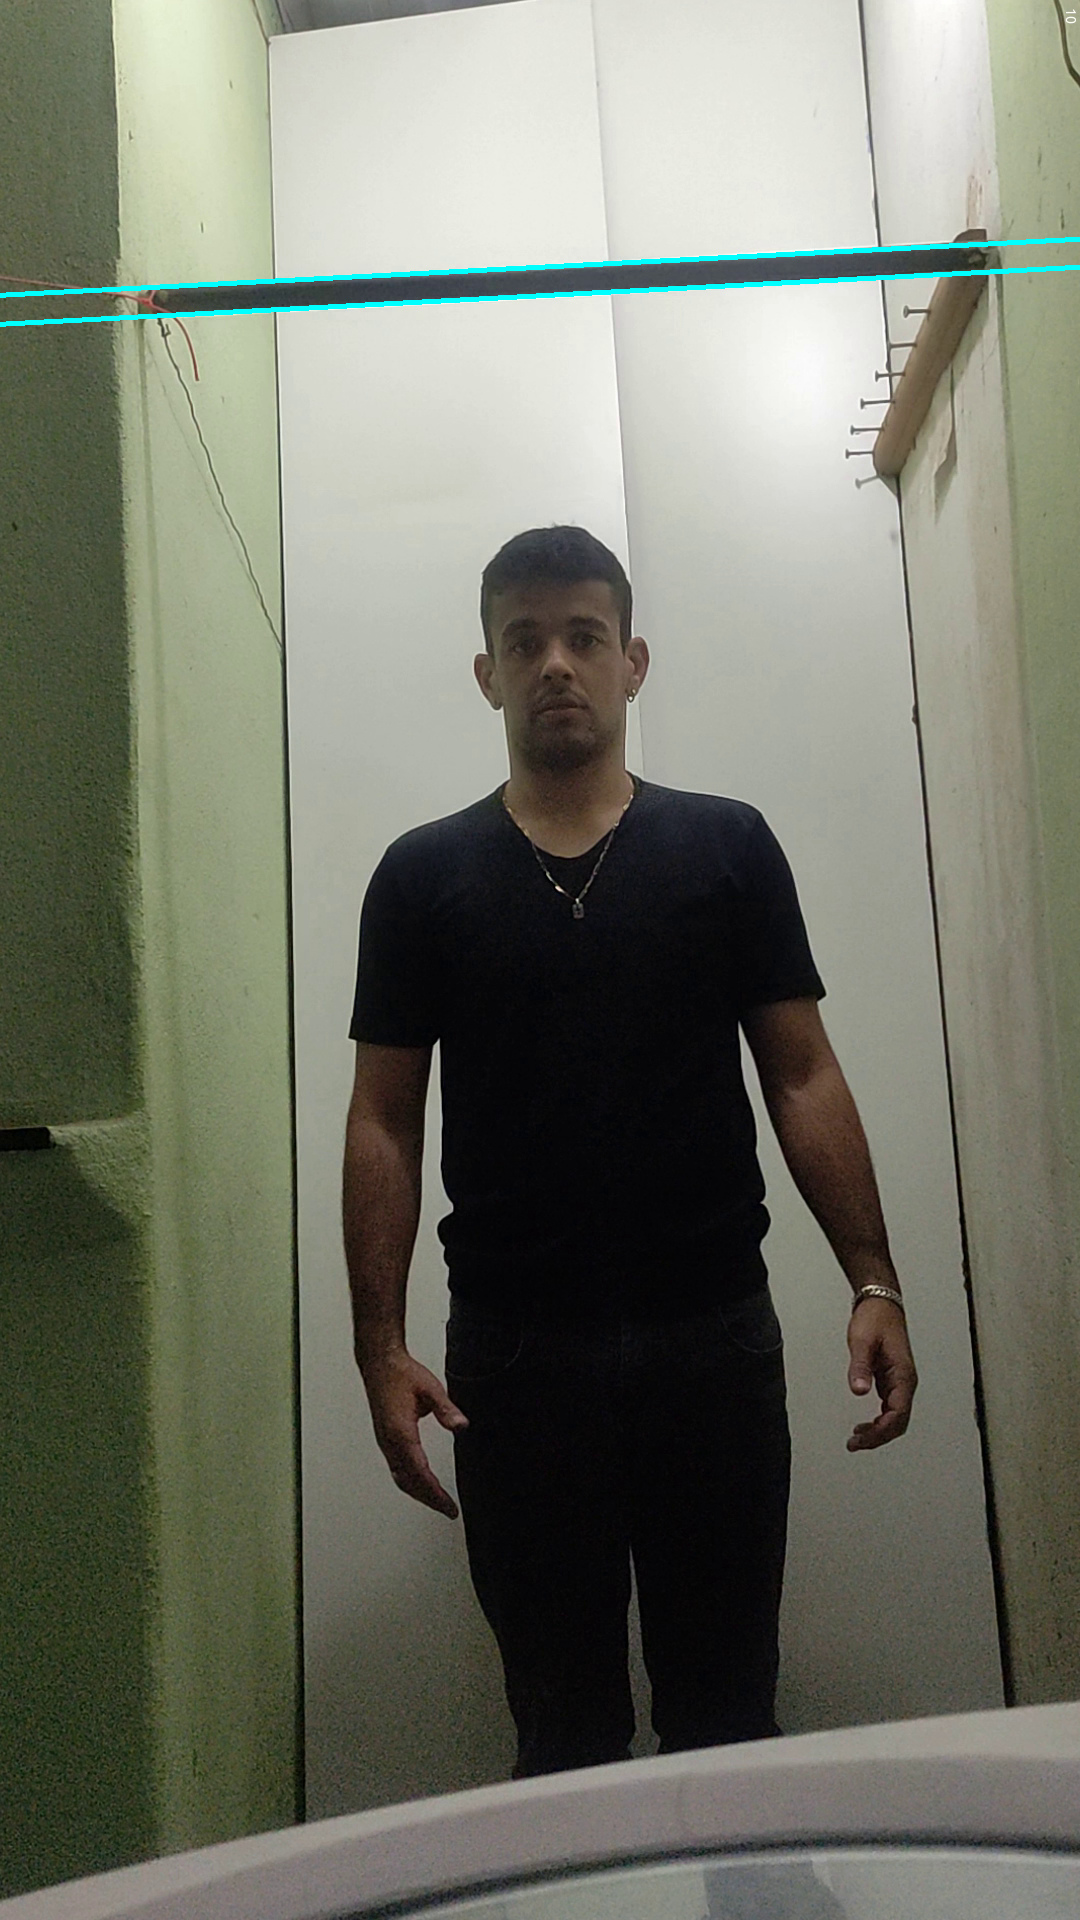
\includegraphics[scale=0.1]{img/desenvolvimento/detectaBarra/barras.png}
    \caption*{Fonte - Próprio Autor.}
    \end{figure}
\end{frame}


\begin{frame}{Detecção da barra - Segmento de Reta Unificado.}
    \begin{figure}[!ht]
    \centering
    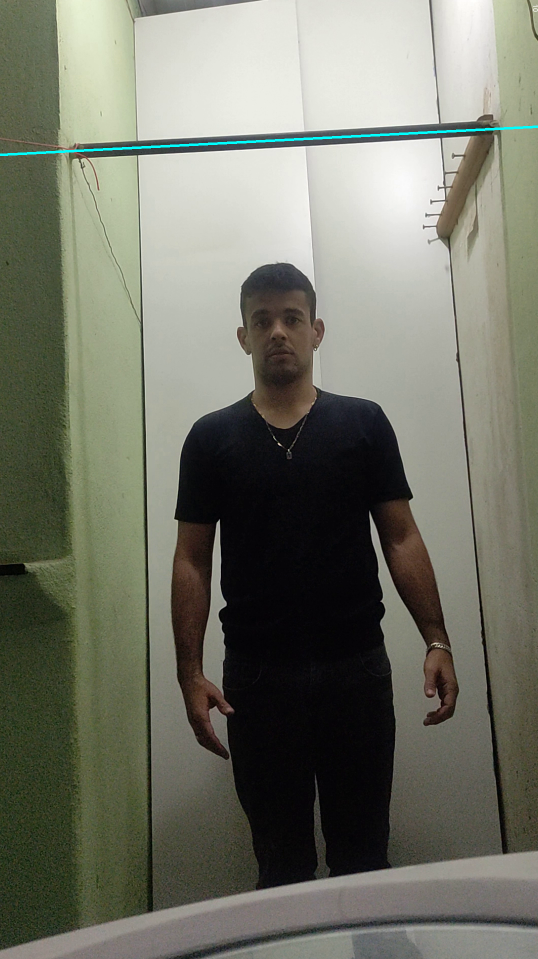
\includegraphics[scale=0.20]{img/desenvolvimento/detectaBarra/barra_unificada.png}
    \caption*{Fonte - Próprio Autor.}
    \end{figure}
\end{frame}

%%%%%%%%%%%%%%%%%%%%%%%%%%%%%%%%%%%%%%%%%%%%%%%%%%%%%%%%%%%%%%%%%%%%
%%
%%                     Inclinação da barra
%%
%%%%%%%%%%%%%%%%%%%%%%%%%%%%%%%%%%%%%%%%%%%%%%%%%%%%%%%%%%%%%%%%%%%%
\begin{frame}{Inclinação da barra}
    \begin{figure}[!ht]
    \centering
    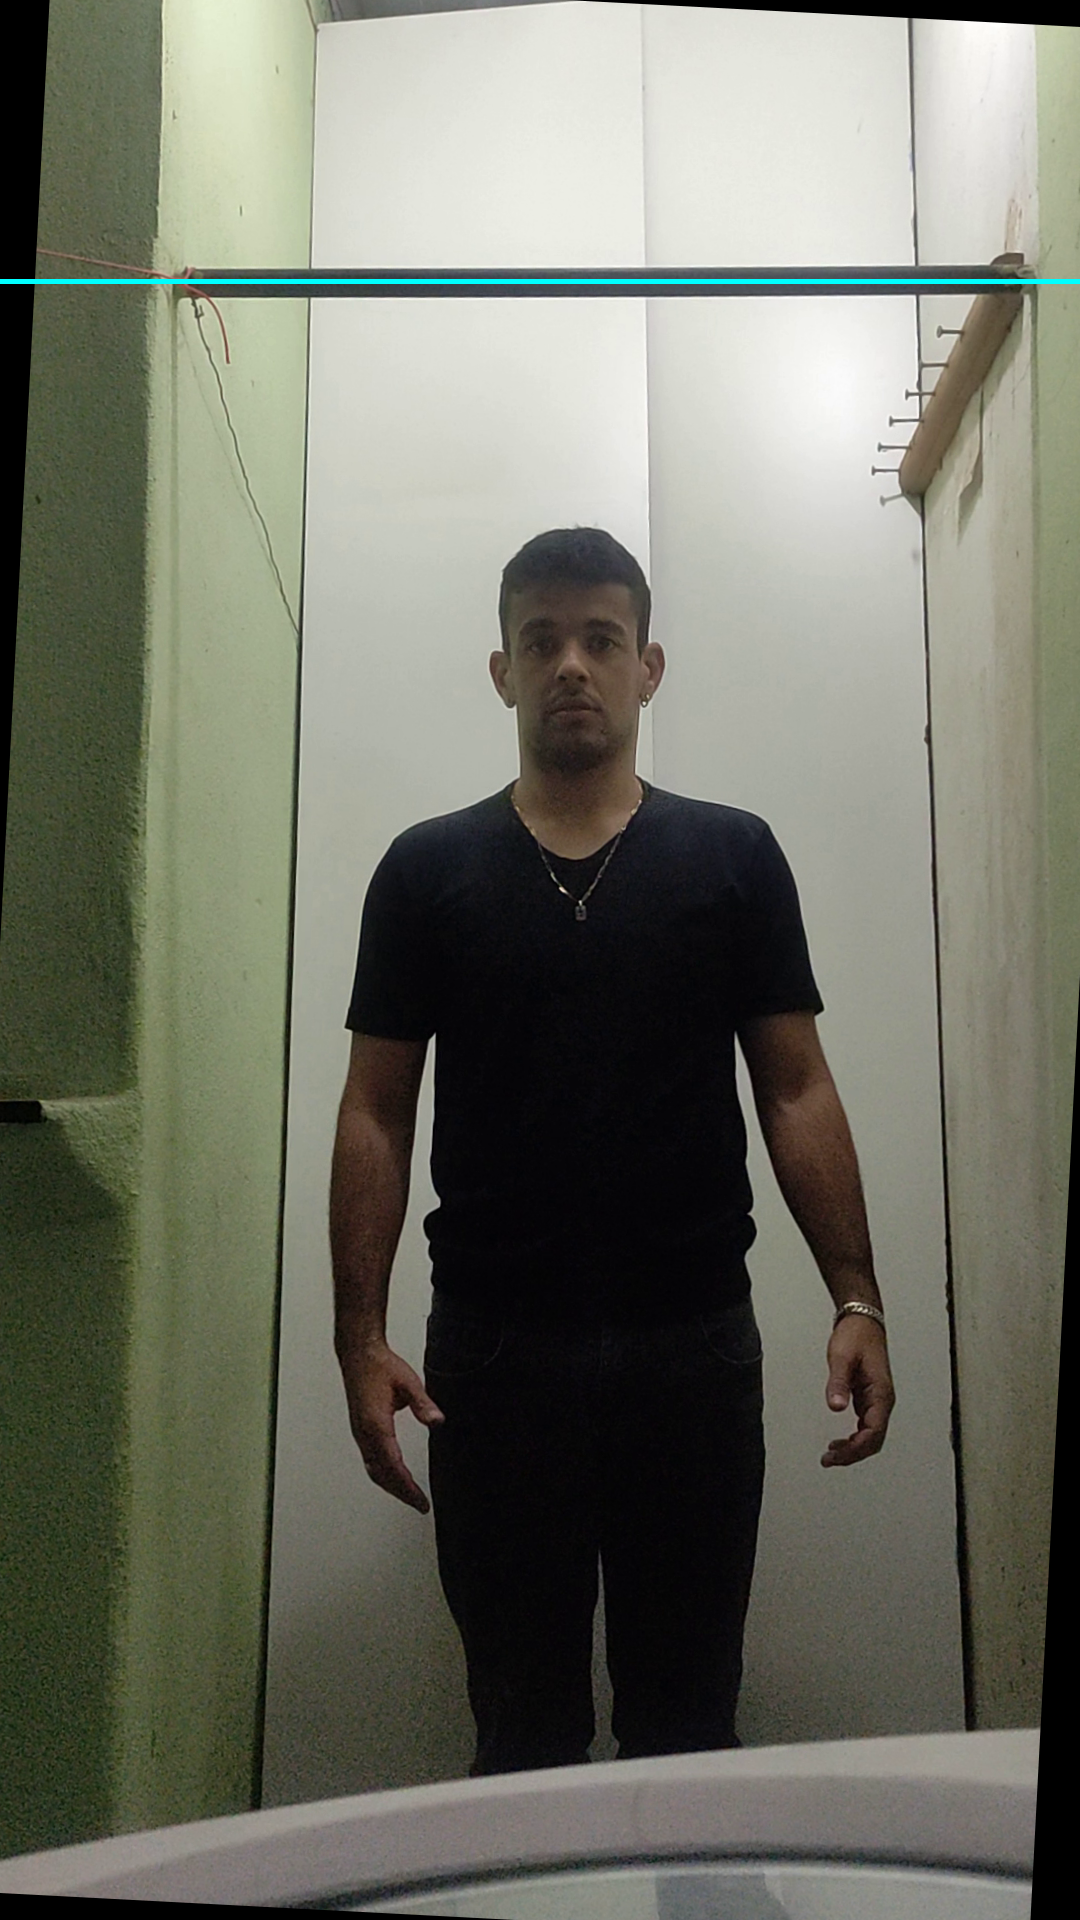
\includegraphics[scale=0.1]{img/desenvolvimento/inclinacaoBarra/barra_rotacionada.png}
    \caption*{Fonte - Próprio Autor.}
    \end{figure}
\end{frame}


%%%%%%%%%%%%%%%%%%%%%%%%%%%%%%%%%%%%%%%%%%%%%%%%%%%%%%%%%%%%%%%%%%%%
%%
%%                     Reconhecimento de pose humana
%%
%%%%%%%%%%%%%%%%%%%%%%%%%%%%%%%%%%%%%%%%%%%%%%%%%%%%%%%%%%%%%%%%%%%%

\begin{frame}{Reconhecimento de pose humana - Pontos chaves}
    \begin{figure}[!ht]
    \centering
    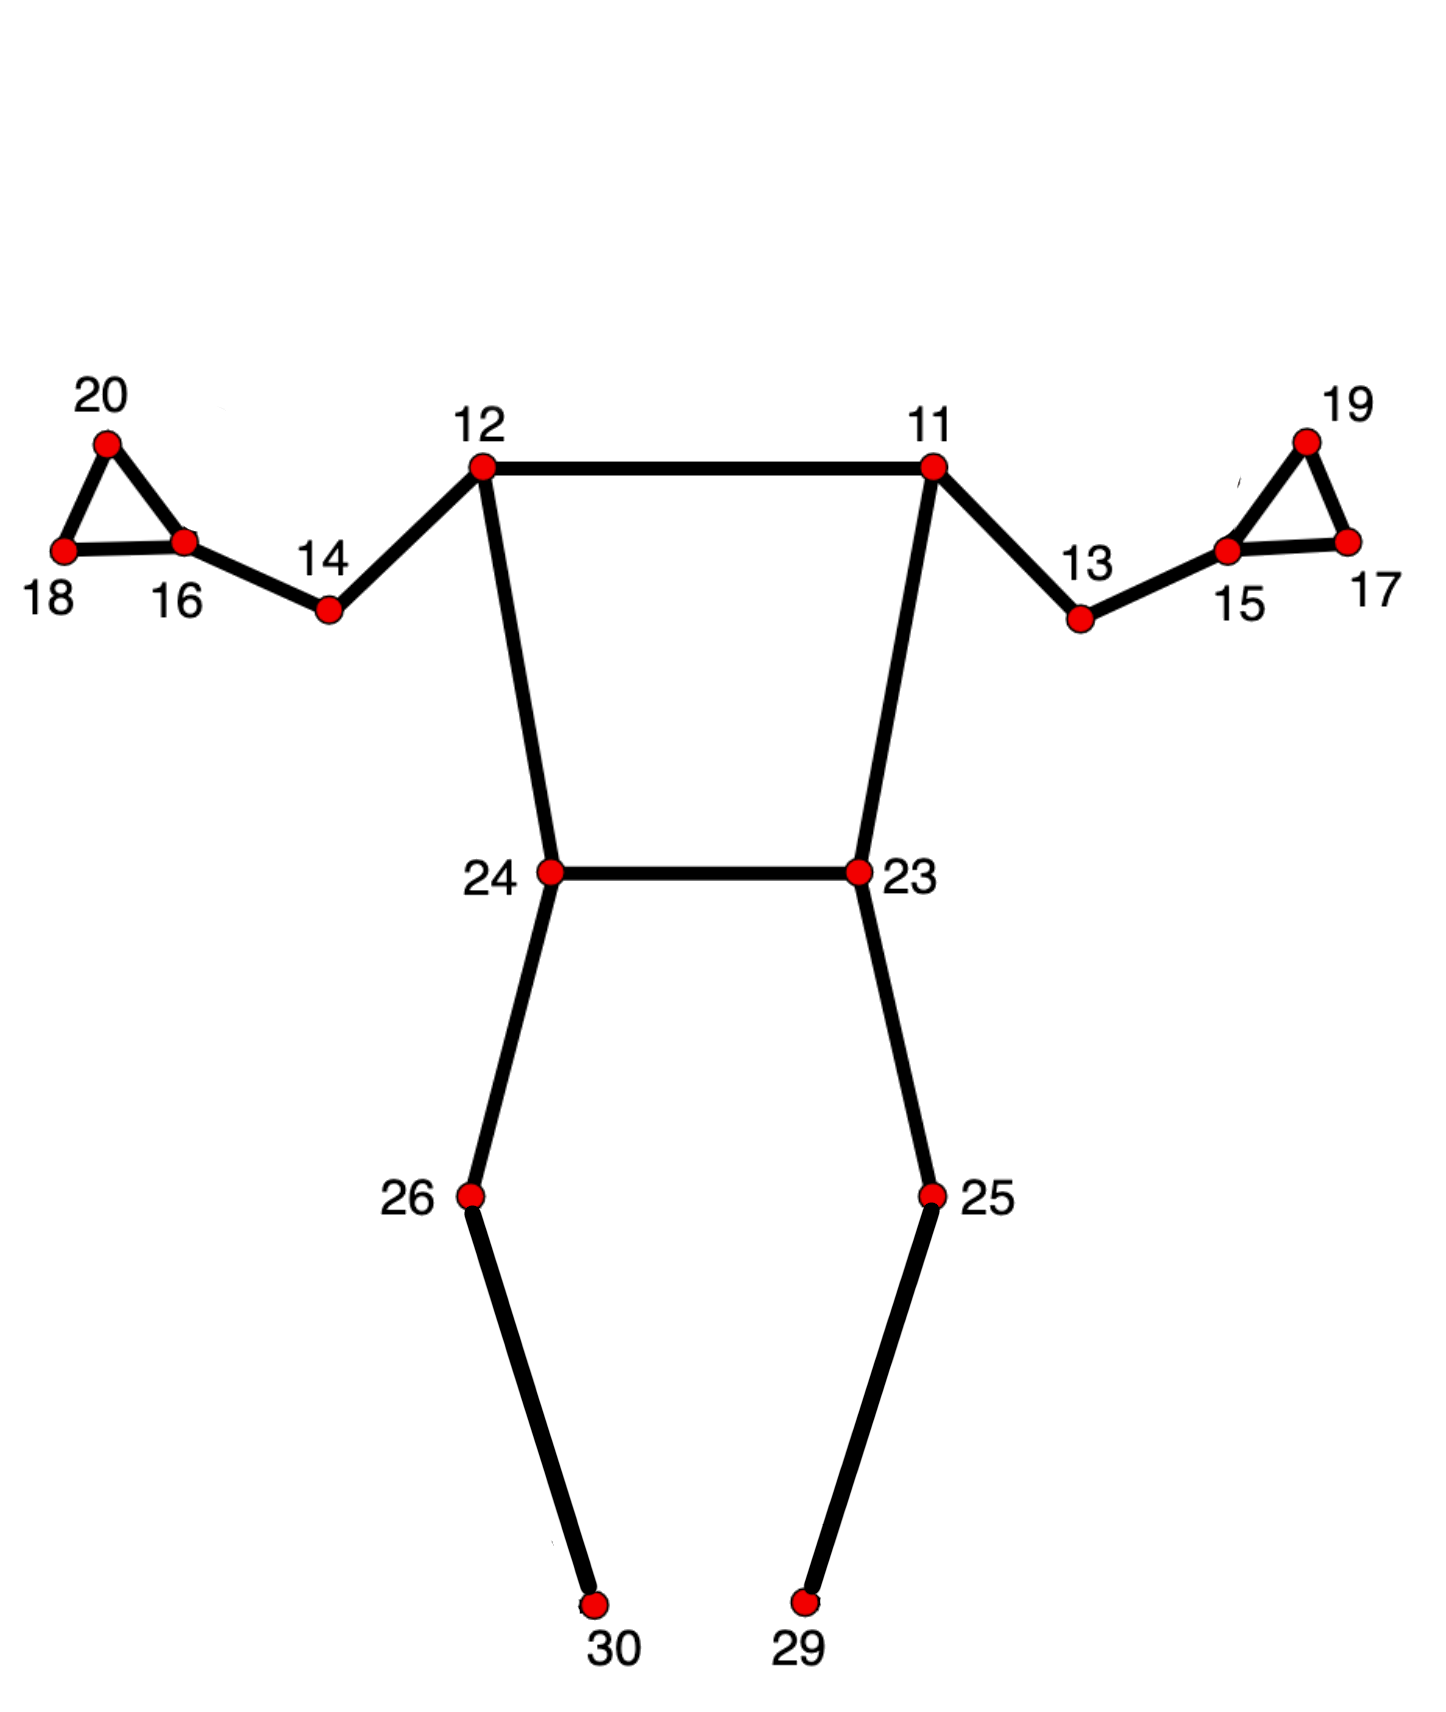
\includegraphics[scale=0.2]{img/desenvolvimento/eph/pose_landmarks_custom.png}
    \caption*{Fonte - Próprio Autor.}
    \end{figure}
\end{frame}

\begin{frame}{Reconhecimento de pose humana }
    \begin{figure}[!ht]
    \centering
    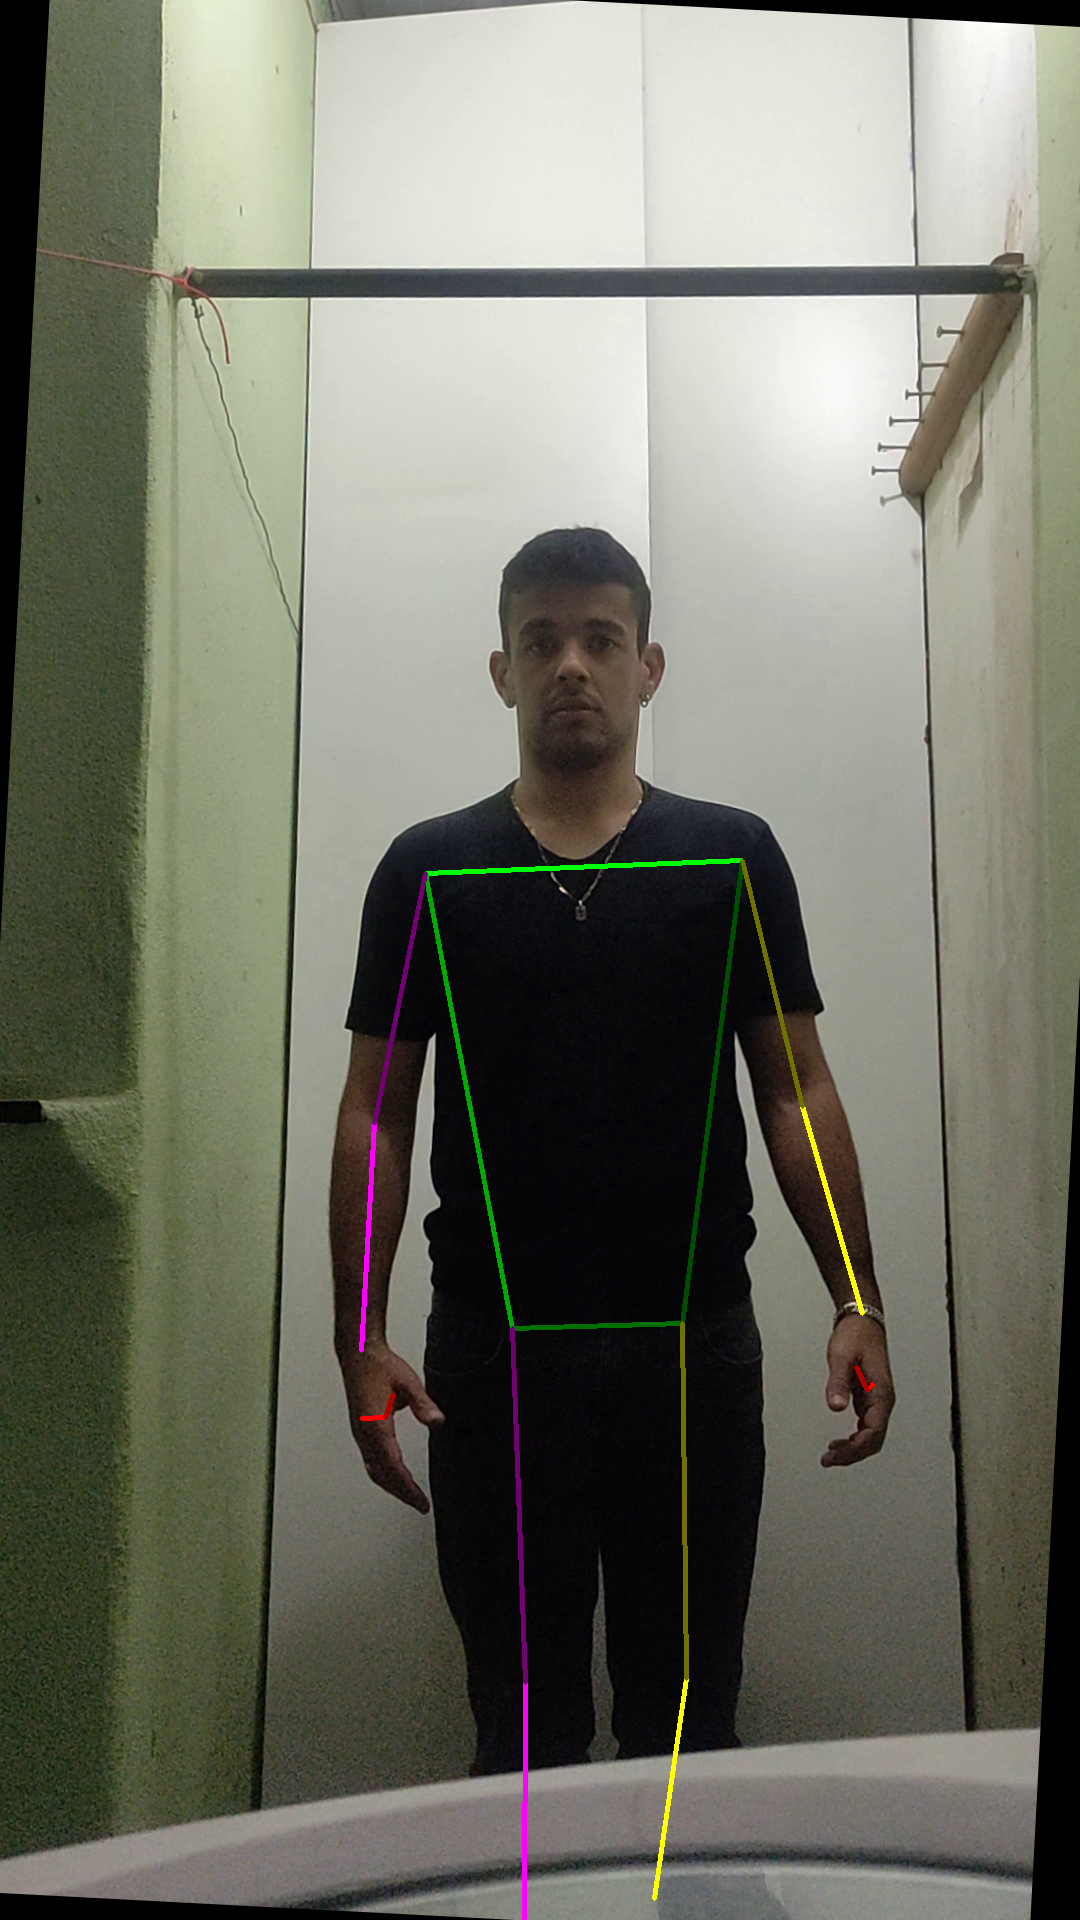
\includegraphics[scale=0.1]{img/desenvolvimento/eph/landmark.png}
    \caption*{Fonte - Próprio Autor.}
    \end{figure}
\end{frame}


%%%%%%%%%%%%%%%%%%%%%%%%%%%%%%%%%%%%%%%%%%%%%%%%%%%%%%%%%%%%%%%%%%%%
%%
%%                     Mão na barra
%%
%%%%%%%%%%%%%%%%%%%%%%%%%%%%%%%%%%%%%%%%%%%%%%%%%%%%%%%%%%%%%%%%%%%%

\begin{frame}{Mão na barra - Fluxograma}
    \begin{figure}[!ht]
    \centering
    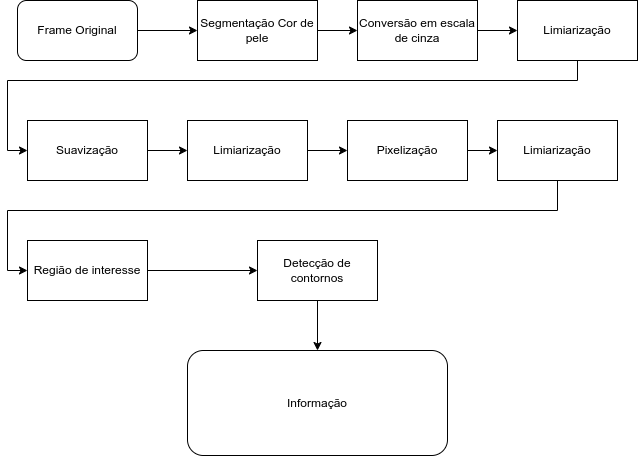
\includegraphics[scale=0.4]{img/desenvolvimento/maoBarra/fluxograma.png}
    \caption*{Fonte - Próprio Autor.}
    \end{figure}
\end{frame}


\begin{frame}{Mão na barra - Imagem original}
    \begin{figure}[!ht]
    \centering
    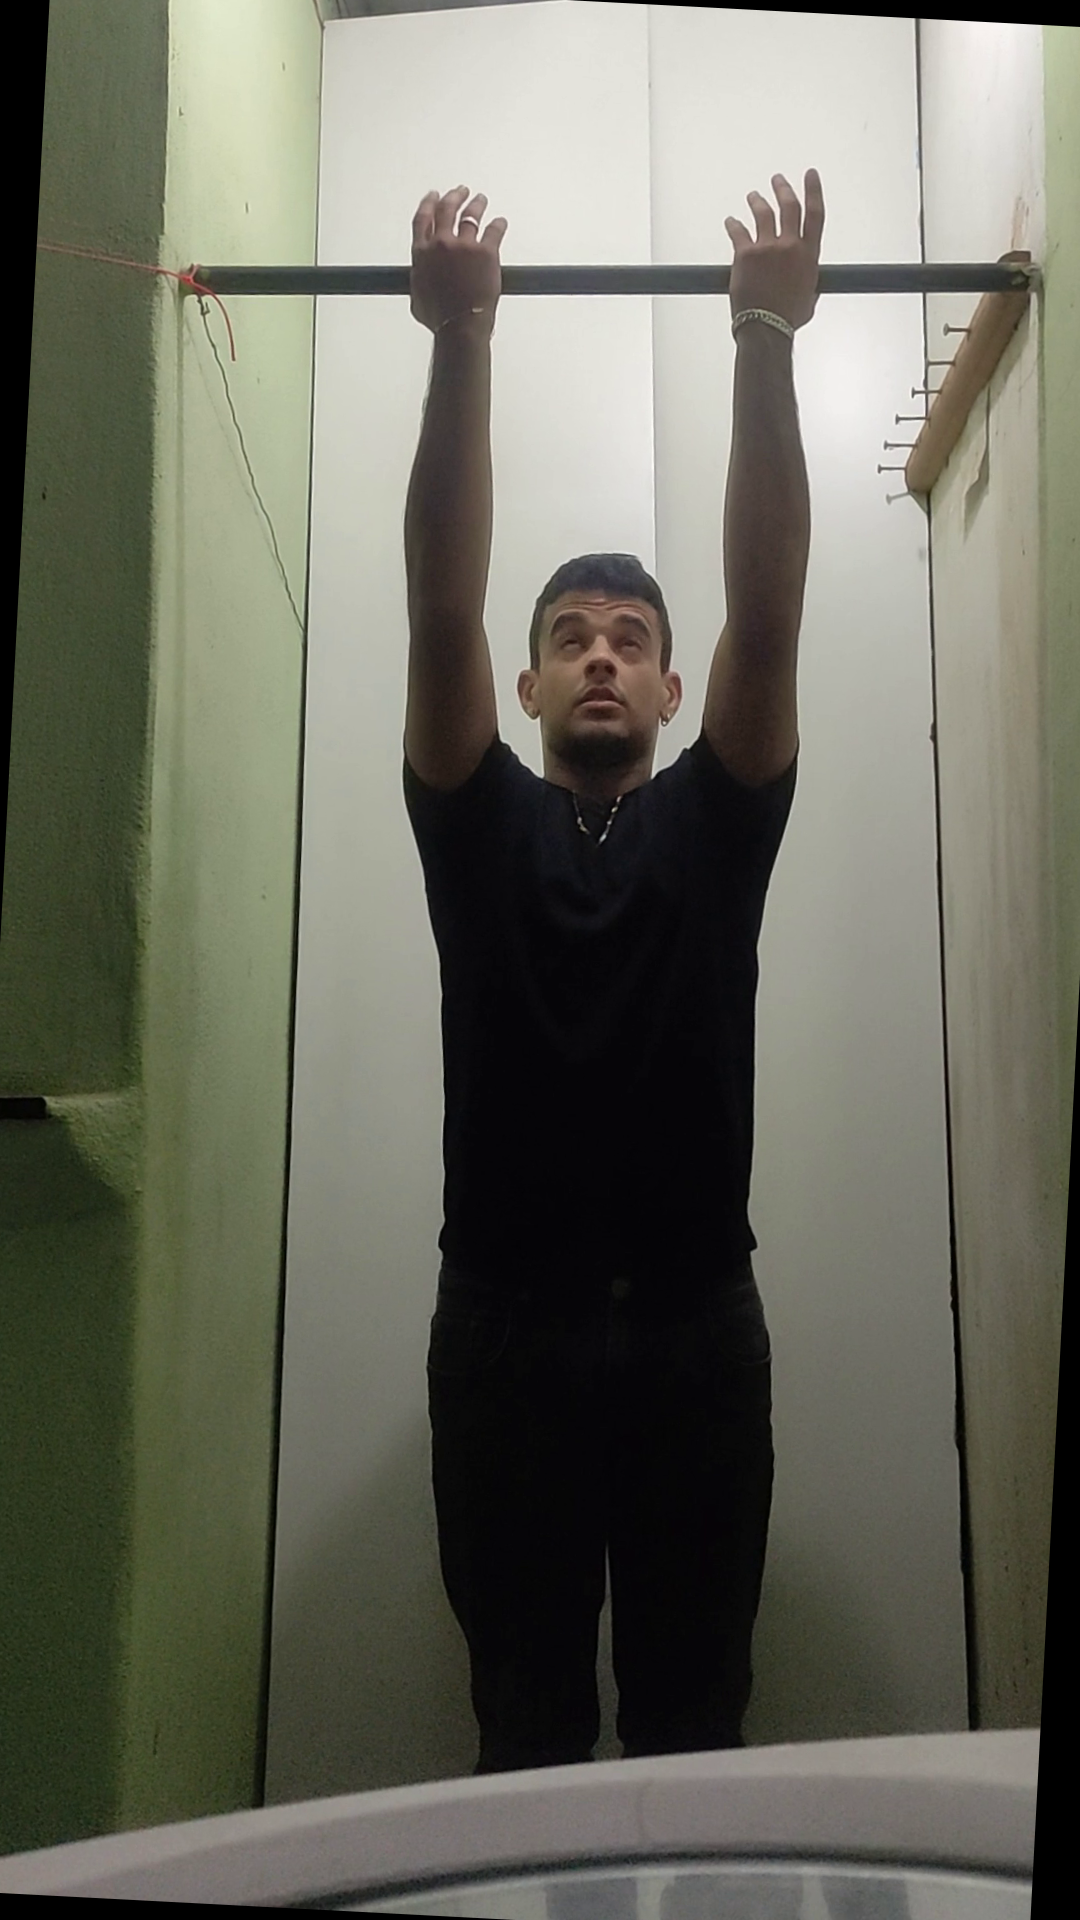
\includegraphics[scale=0.1]{img/desenvolvimento/maoBarra/original.png}
    \caption*{Fonte - Próprio Autor.}
    \end{figure}
\end{frame}


\begin{frame}{Mão na barra - Filtro cor de pele}
    \begin{figure}[!ht]
    \centering
    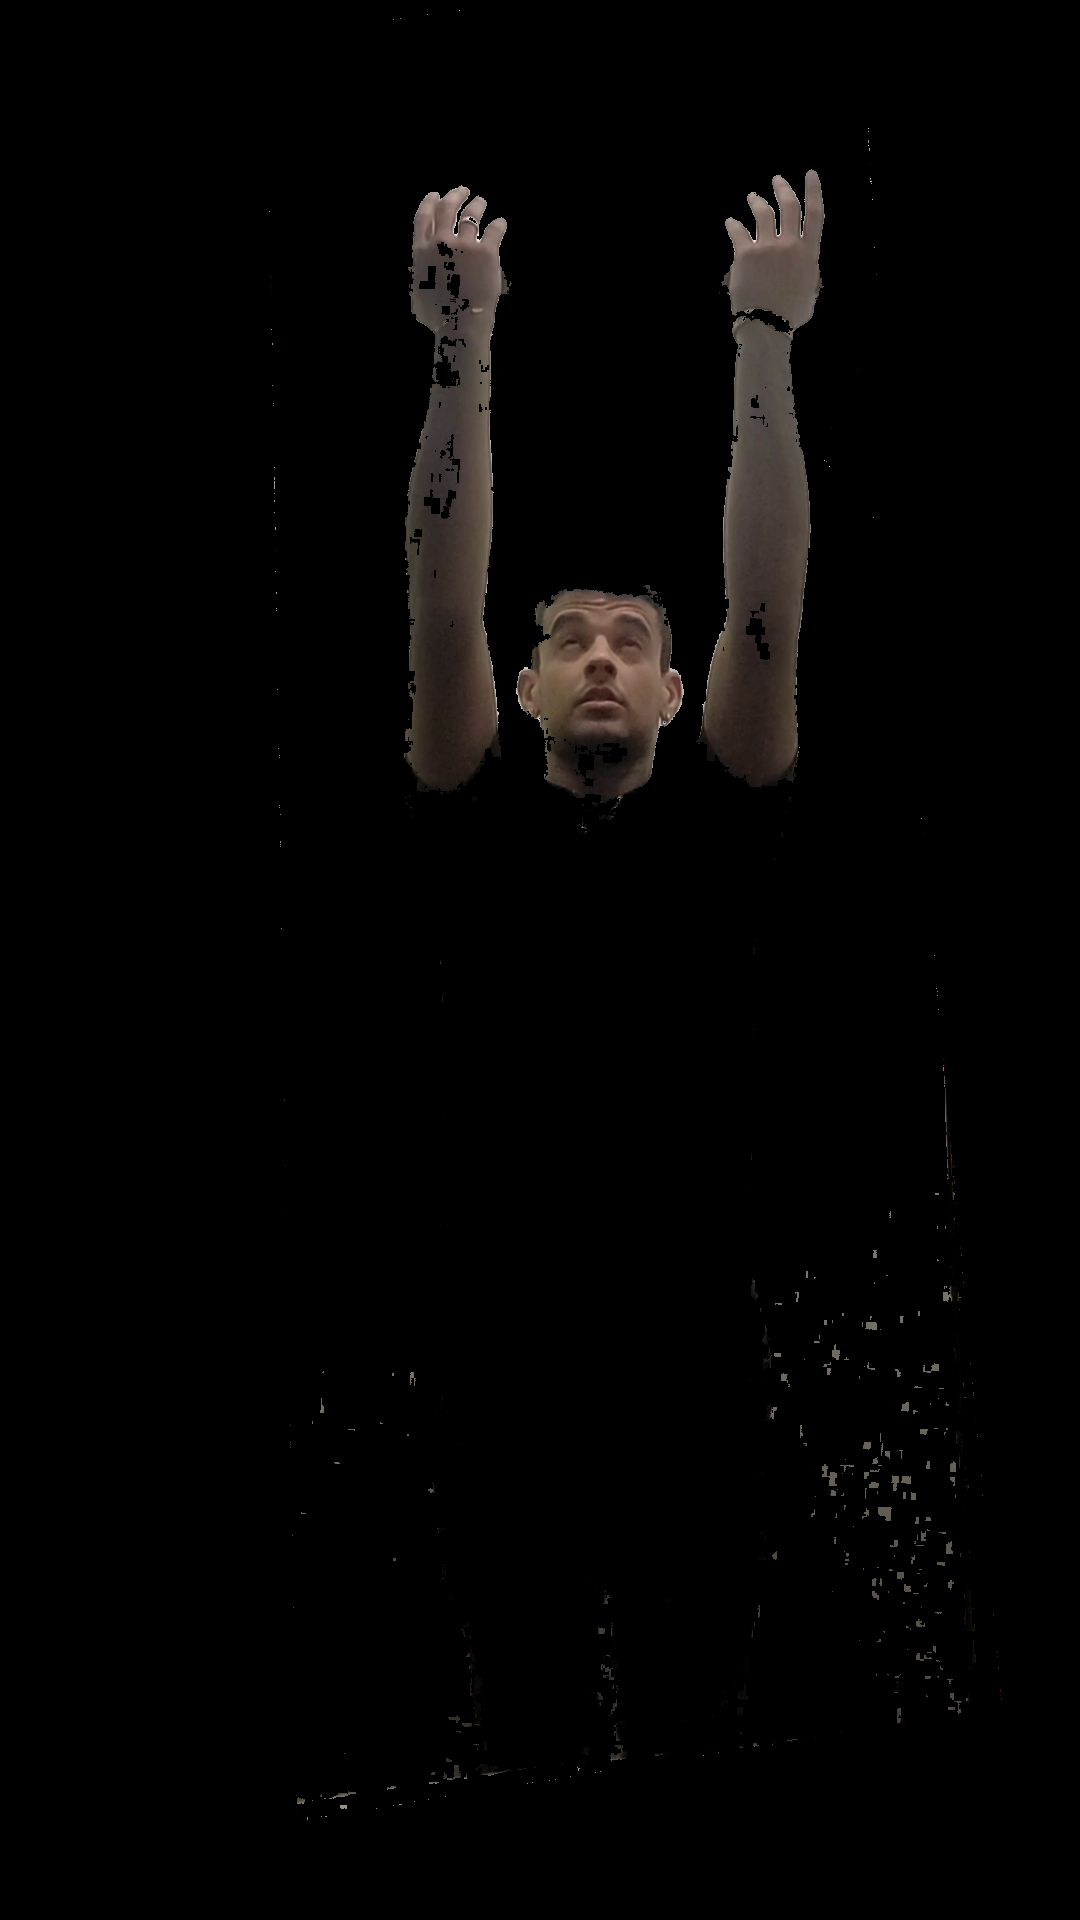
\includegraphics[scale=0.1]{img/desenvolvimento/maoBarra/skin.png}
    \caption*{Fonte - Próprio Autor.}
    \end{figure}
\end{frame}


\begin{frame}{Mão na barra - Escala de cinza}
    \begin{figure}[!ht]
    \centering
    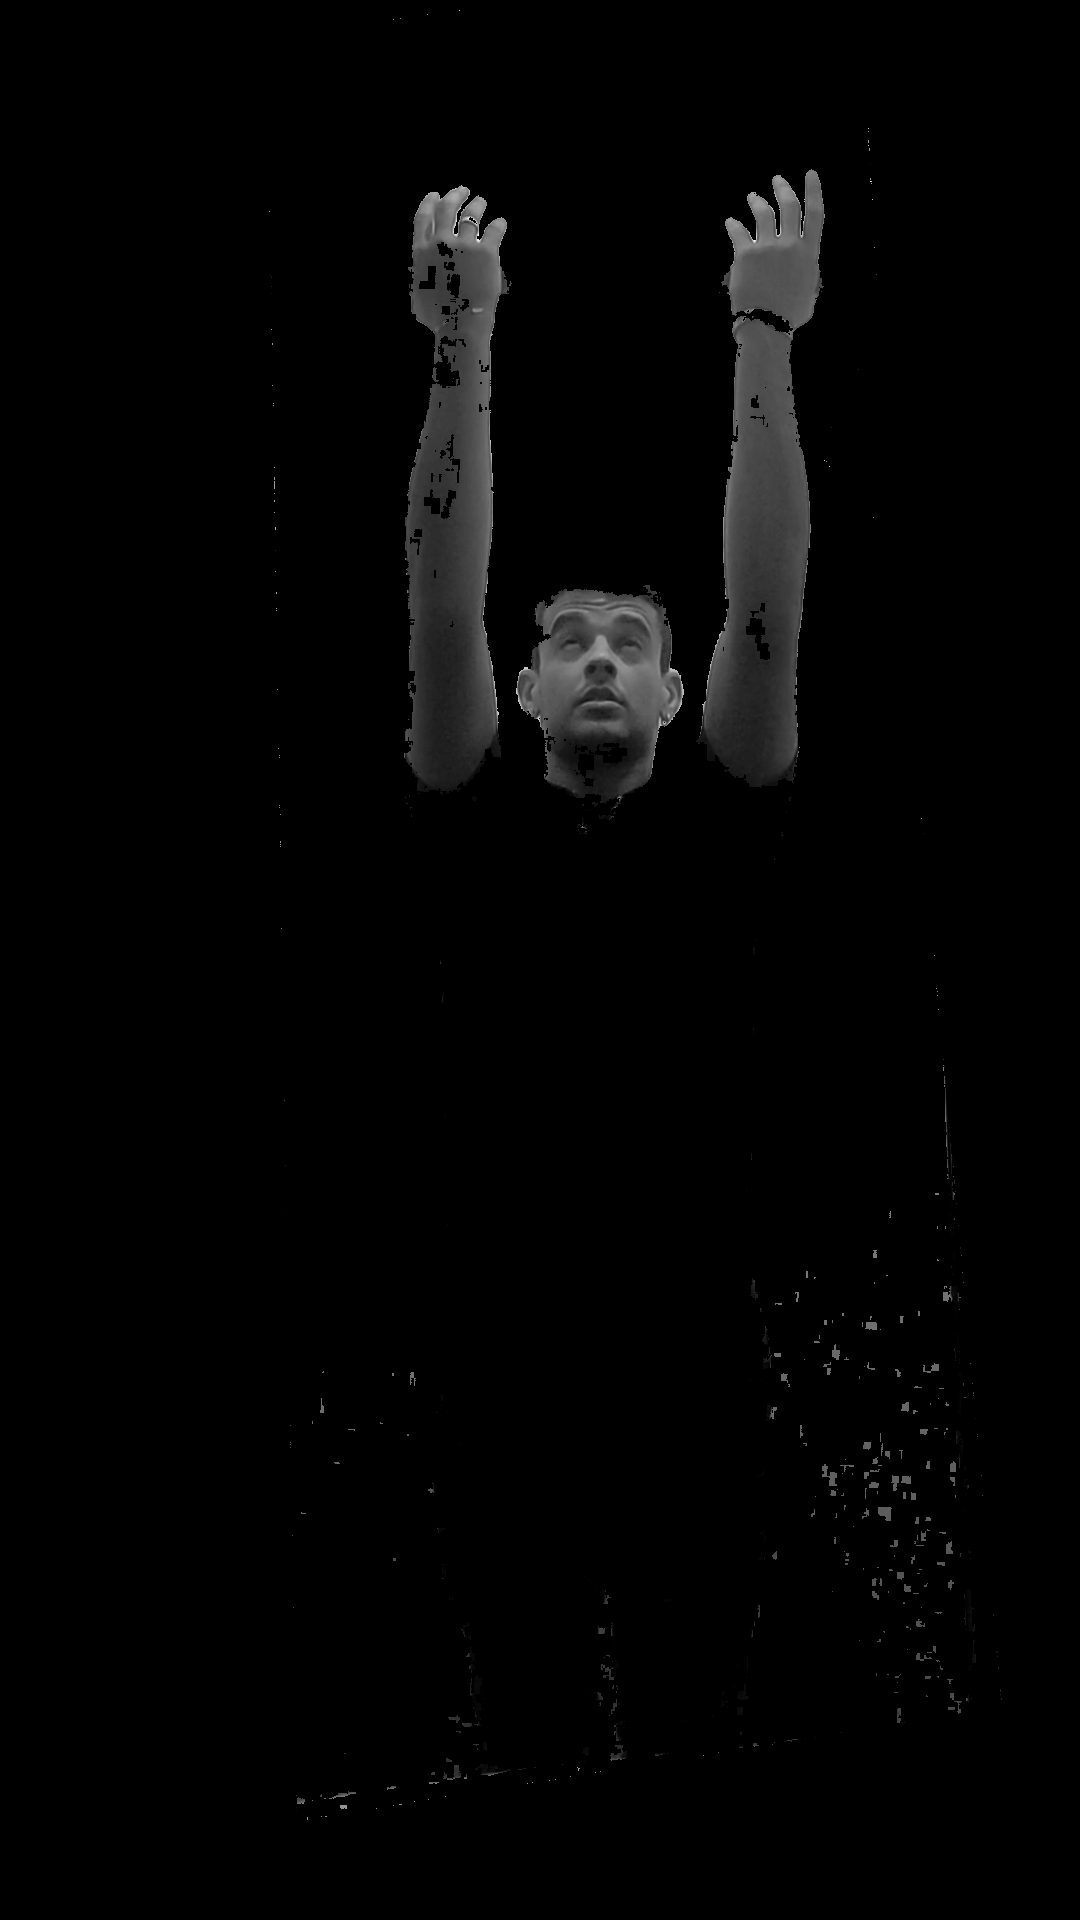
\includegraphics[scale=0.1]{img/desenvolvimento/maoBarra/gray.png}
    \caption*{Fonte - Próprio Autor.}
    \end{figure}
\end{frame}

\begin{frame}{Mão na barra - Limiarização}
    \begin{figure}[!ht]
    \centering
    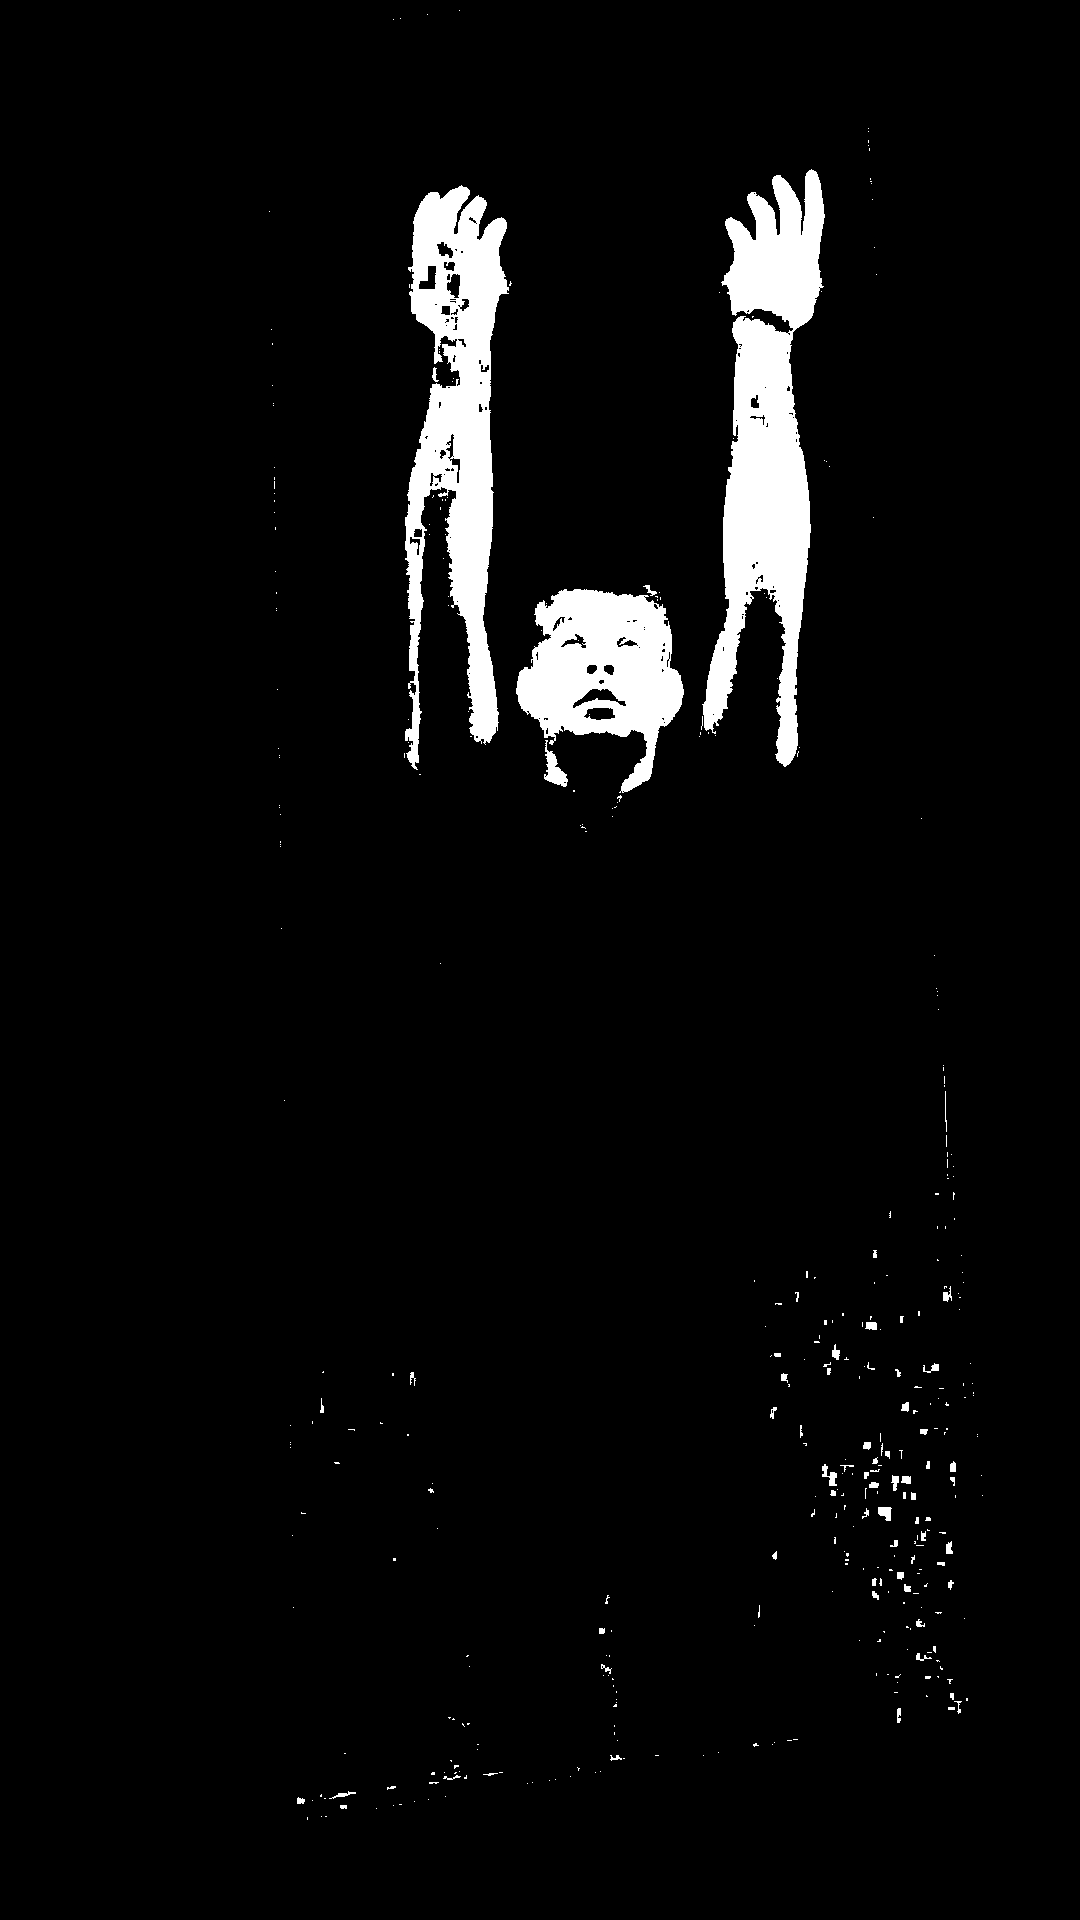
\includegraphics[scale=0.1]{img/desenvolvimento/maoBarra/limited.png}
    \caption*{Fonte - Próprio Autor.}
    \end{figure}
\end{frame}


\begin{frame}{Mão na barra - Desfoque}
    \begin{figure}[!ht]
    \centering
    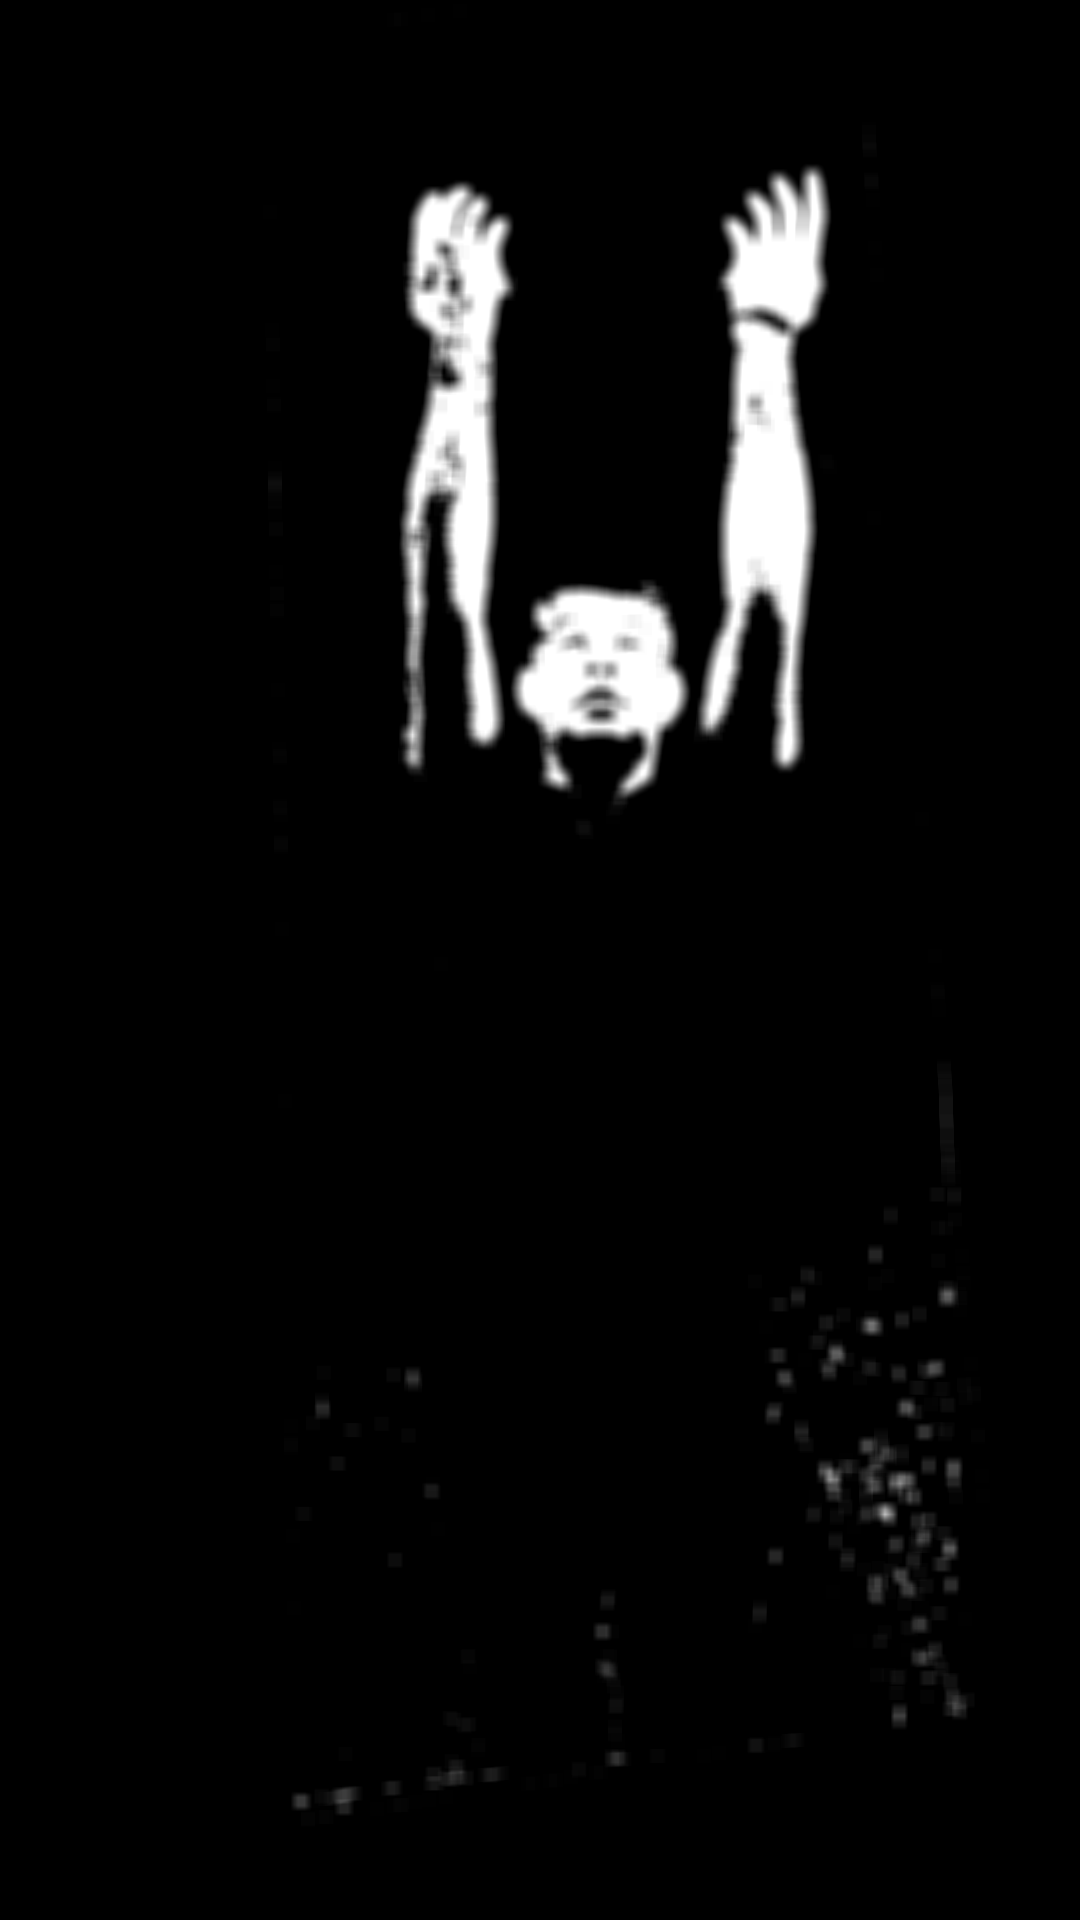
\includegraphics[scale=0.1]{img/desenvolvimento/maoBarra/blur.png}
    \caption*{Fonte - Próprio Autor.}
    \end{figure}
\end{frame}


\begin{frame}{Mão na barra - 2º Limiarização}
    \begin{figure}[!ht]
    \centering
    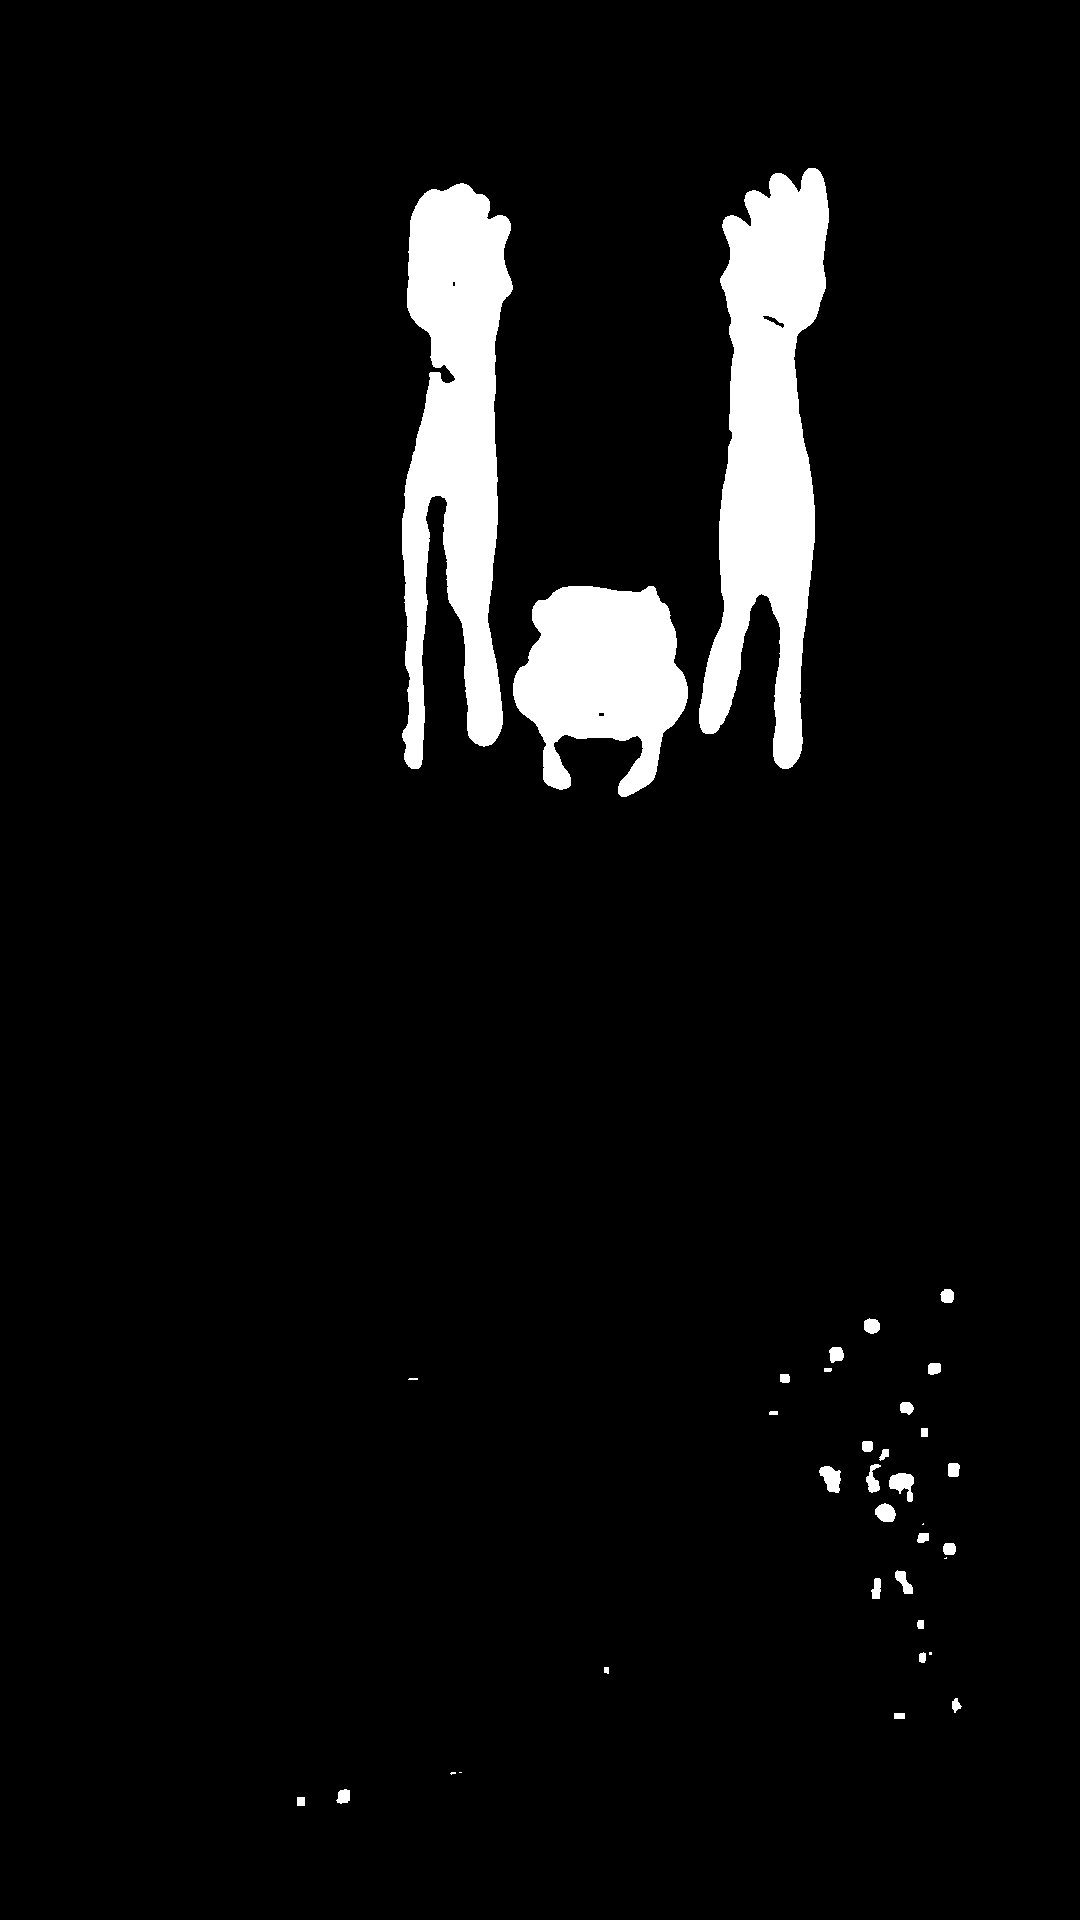
\includegraphics[scale=0.1]{img/desenvolvimento/maoBarra/limited2.png}
    \caption*{Fonte - Próprio Autor.}
    \end{figure}
\end{frame}

\begin{frame}{Mão na barra - Pixel}
    \begin{figure}[!ht]
    \centering
    
\includegraphics[scale=0.1]{img/desenvolvimento/maoBarra/pixel.png}
    \caption*{Fonte - Próprio Autor.}
    \end{figure}
\end{frame}


\begin{frame}{Mão na barra - 3º Limiarização}
    \begin{figure}[!ht]
    \centering
    
\includegraphics[scale=0.1]{img/desenvolvimento/maoBarra/limited3.png}
    \caption*{Fonte - Próprio Autor.}
    \end{figure}
\end{frame}

\begin{frame}{Mão na barra - Máscara da região de interesse}
    \begin{figure}[!ht]
    \centering
    
\includegraphics[scale=0.1]{img/desenvolvimento/maoBarra/mask3.png}
    \caption*{Fonte - Próprio Autor.}
    \end{figure}
\end{frame}

\begin{frame}{Mão na barra - Imagem segmentada}
    \begin{figure}[!ht]
    \centering
    
\includegraphics[scale=0.1]{img/desenvolvimento/maoBarra/only_hands.png}
    \caption*{Fonte - Próprio Autor.}
    \end{figure}
\end{frame}


\begin{frame}{Mão na barra - Representação}
    \begin{figure}[!ht]
    \centering
    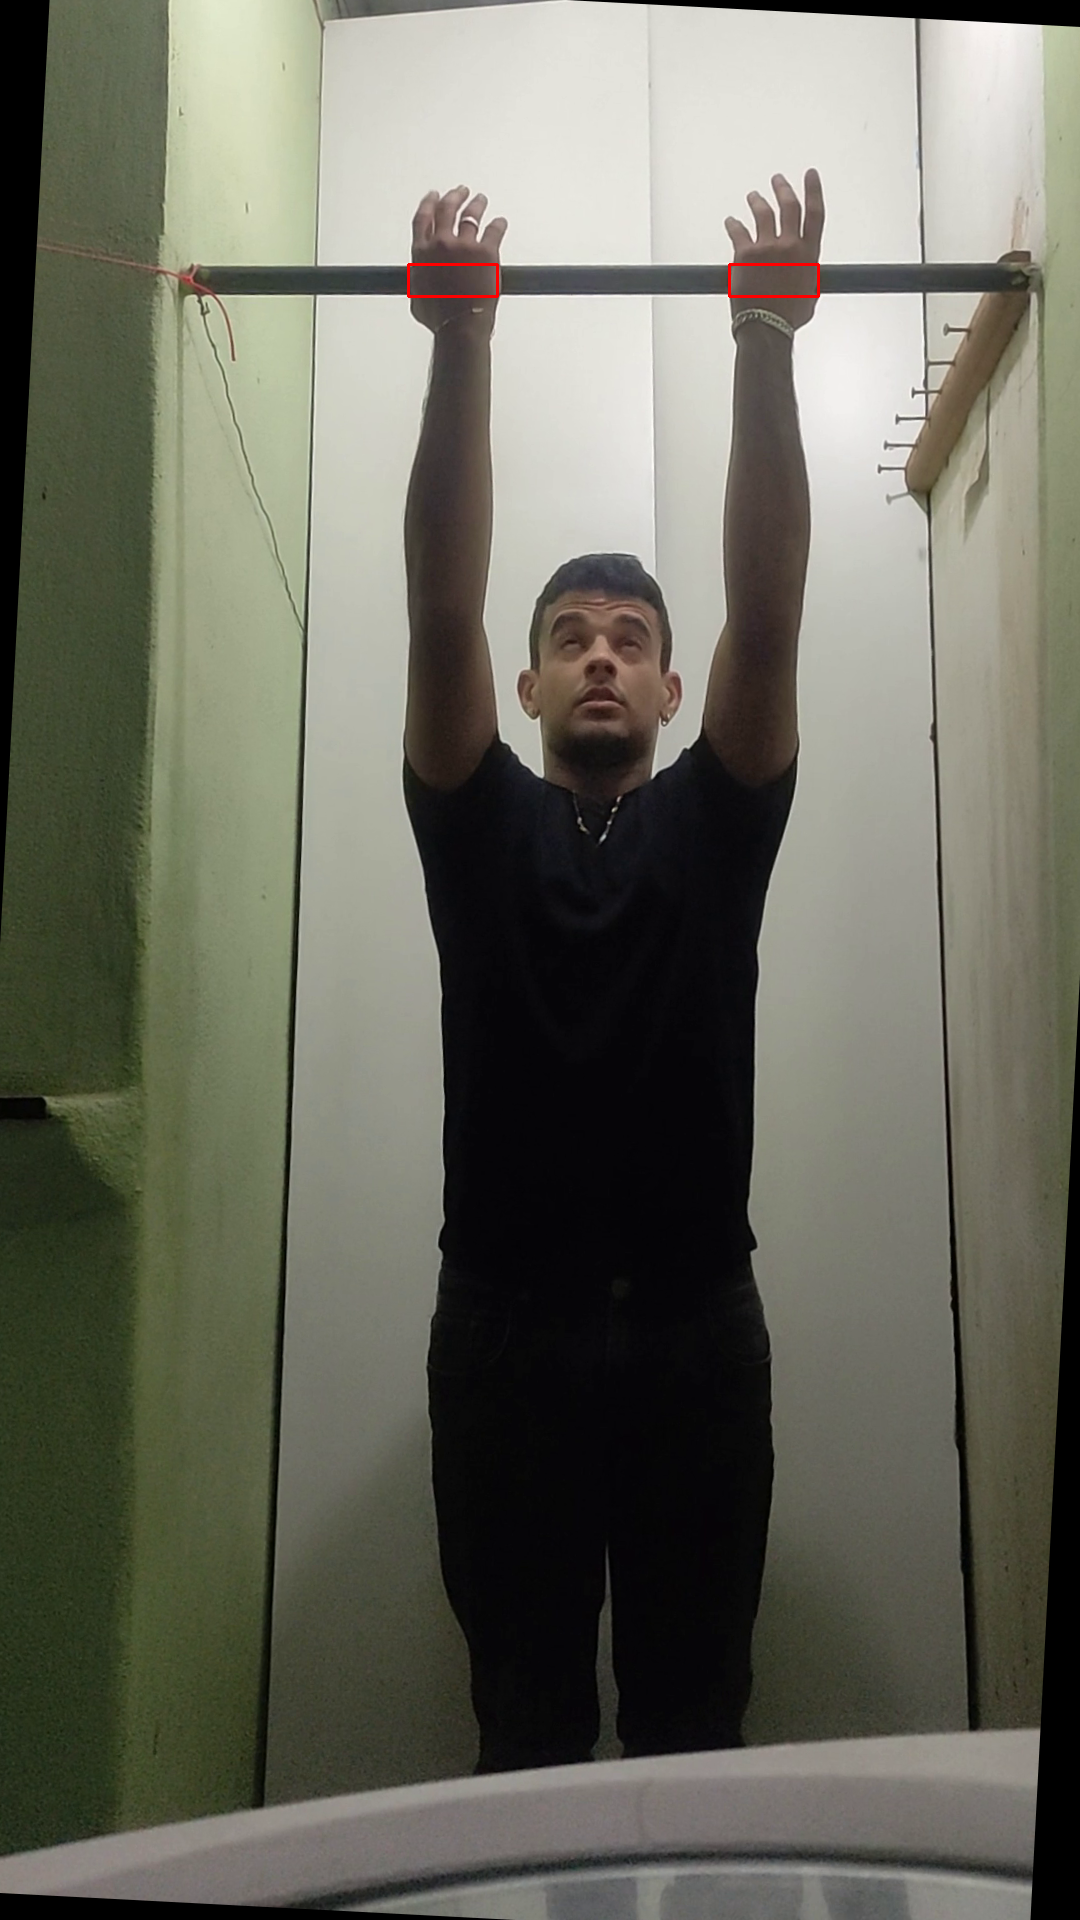
\includegraphics[scale=0.1]{img/desenvolvimento/maoBarra/contornos.png}
    \caption*{Fonte - Próprio Autor.}
    \end{figure}
\end{frame}



%%%%%%%%%%%%%%%%%%%%%%%%%%%%%%%%%%%%%%%%%%%%%%%%%%%%%%%%%%%%%%%%%%%%
%%
%%                     Braço esticado
%%
%%%%%%%%%%%%%%%%%%%%%%%%%%%%%%%%%%%%%%%%%%%%%%%%%%%%%%%%%%%%%%%%%%%%


\begin{frame}{Braço esticado - Fluxograma}
    \begin{figure}[!ht]
        \centering
            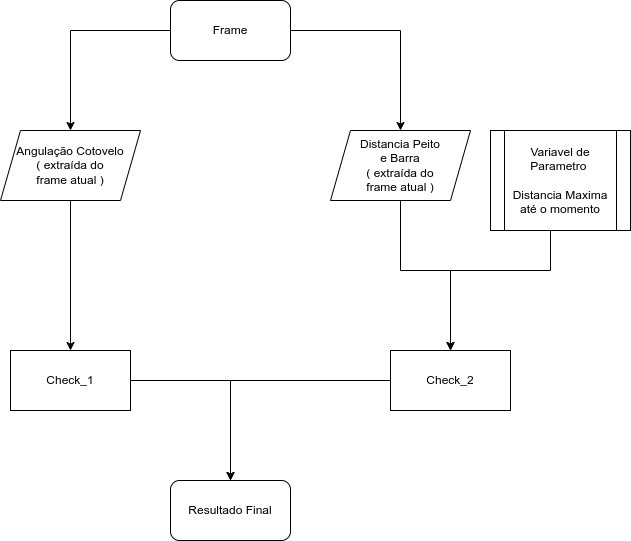
\includegraphics[scale=0.35]{img/desenvolvimento/bracoEsticado/fluxograma.png}
        \caption*{Fonte - Próprio Autor.}
    \end{figure}
\end{frame}


\begin{frame}{Braço esticado - Segmento dos membros}
    \begin{figure}[!ht]
        \centering
            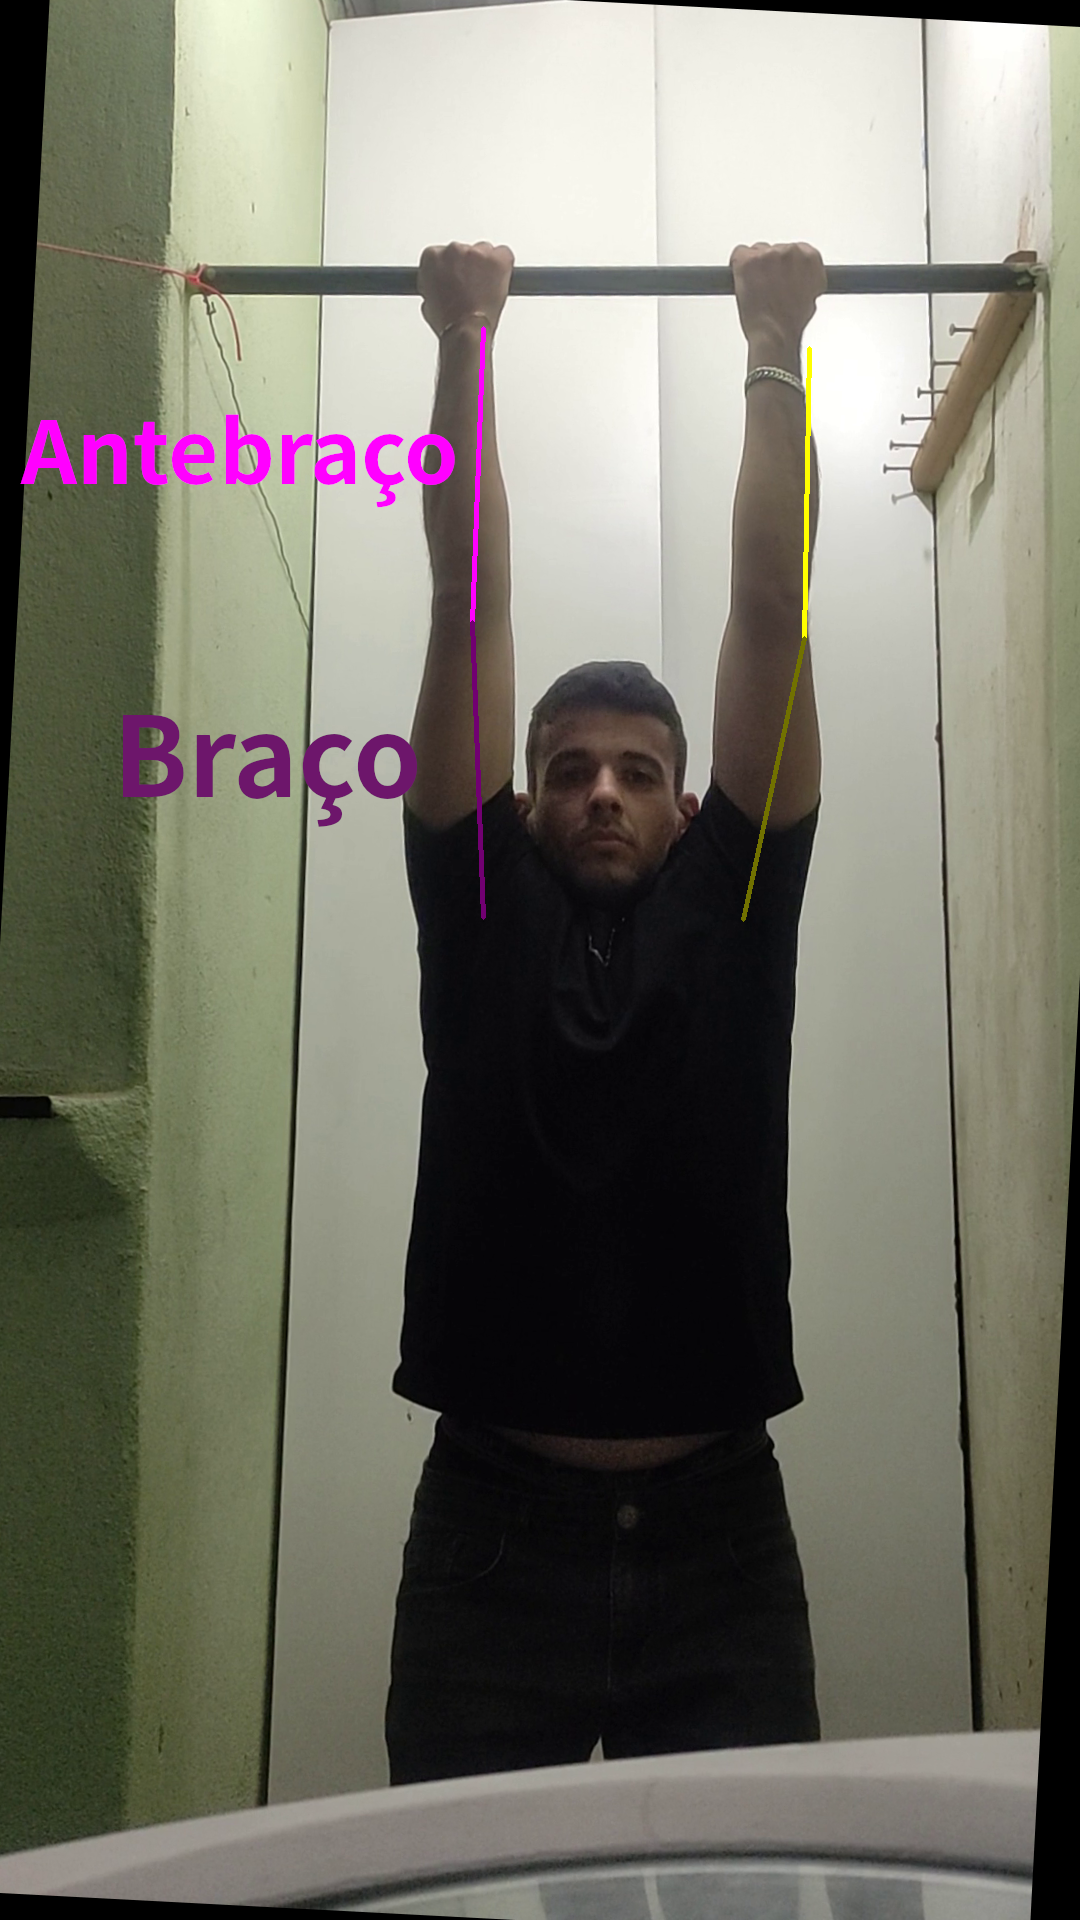
\includegraphics[scale=0.1]{img/desenvolvimento/bracoEsticado/bracoEsticado.png}
        \caption*{Fonte - Próprio Autor.}
    \end{figure}
\end{frame}

\begin{frame}{Braço esticado - Imprecisão}
    \begin{itemize}
        \item É aceito até 13 graus de movimento.
    \end{itemize}
\end{frame}

\begin{frame}{Braço esticado - Ombros}
    \begin{figure}[!ht]
        \centering
            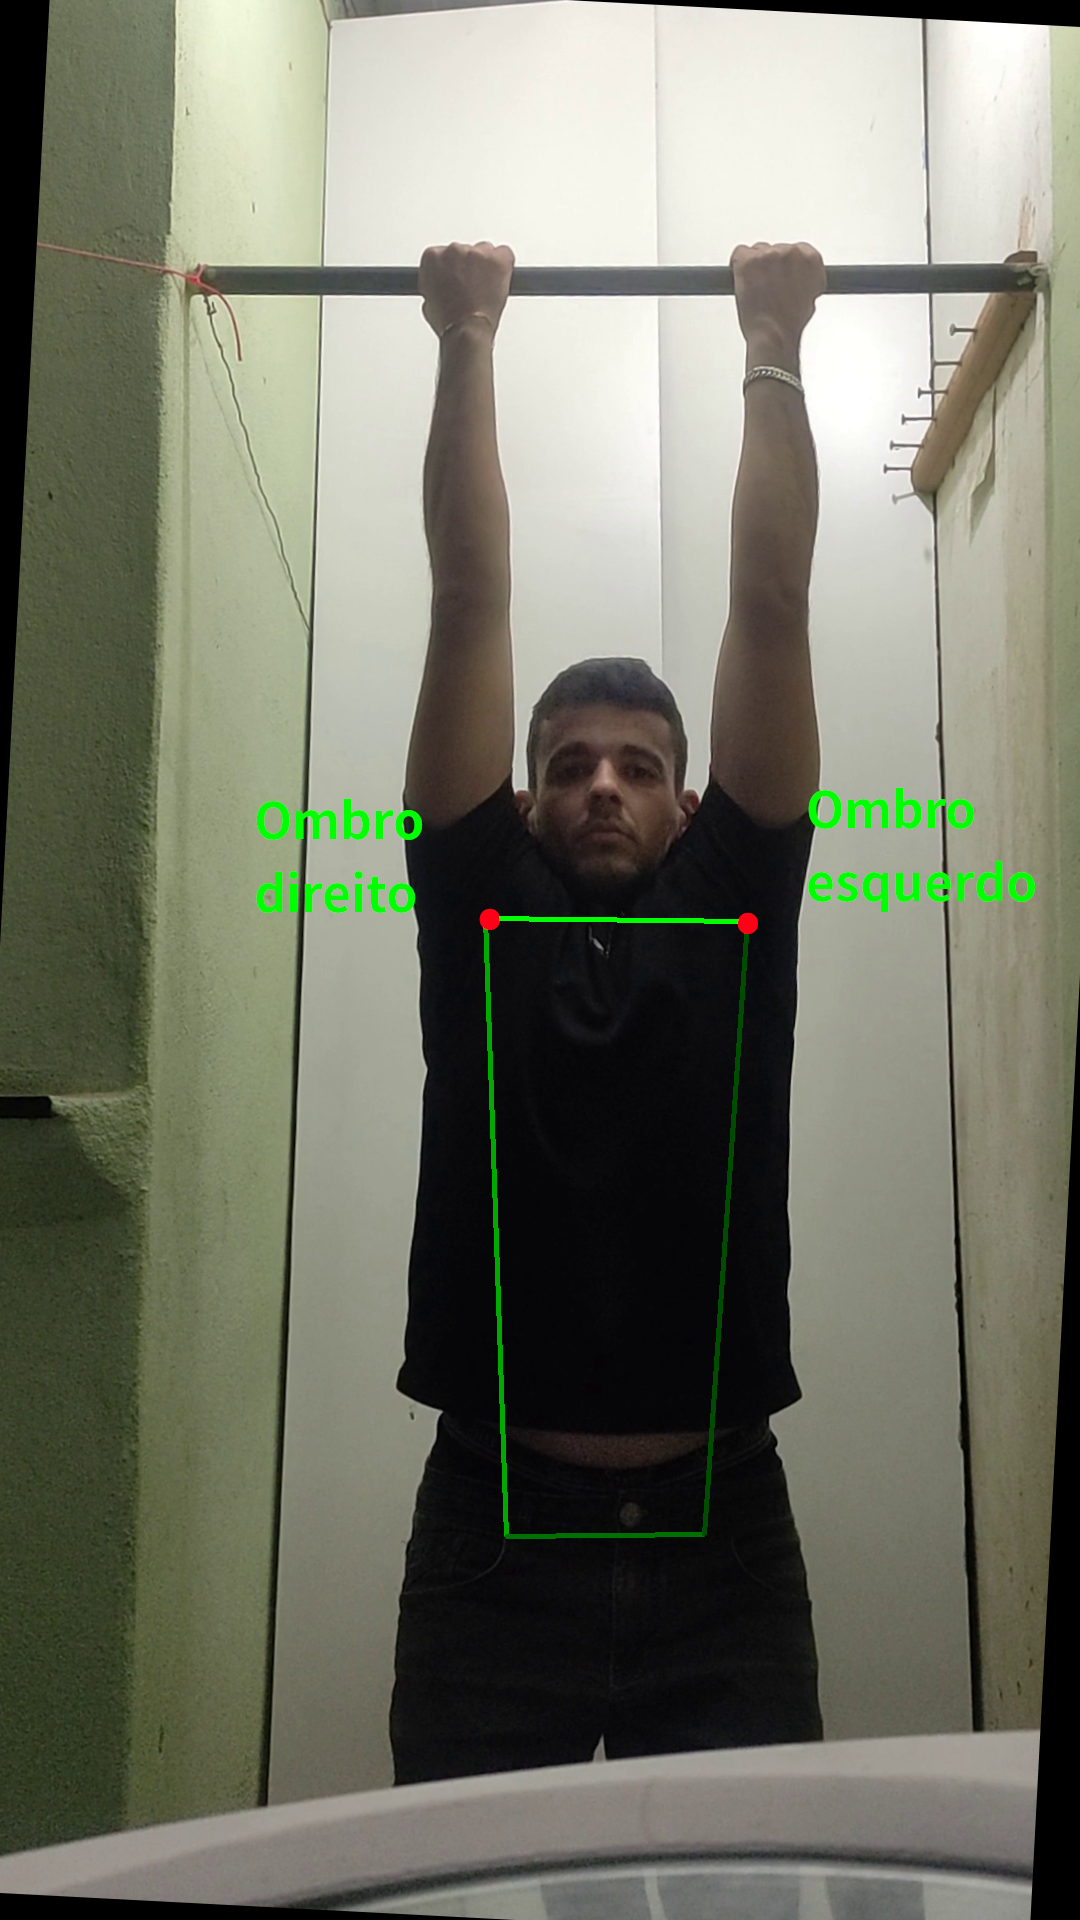
\includegraphics[scale=0.1]{img/desenvolvimento/bracoEsticado/tronco.png}
        \caption*{Fonte - Próprio Autor.}
    \end{figure}
\end{frame}



%%%%%%%%%%%%%%%%%%%%%%%%%%%%%%%%%%%%%%%%%%%%%%%%%%%%%%%%%%%%%%%%%%%%
%%
%%                     Ultrapassagem do queixo a barra
%%
%%%%%%%%%%%%%%%%%%%%%%%%%%%%%%%%%%%%%%%%%%%%%%%%%%%%%%%%%%%%%%%%%%%%

\begin{frame}{Ultrapassagem do queixo à barra - Fluxograma}
    \begin{figure}[!ht]
        \centering
            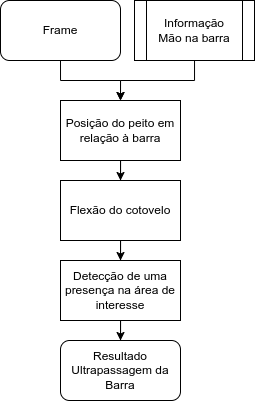
\includegraphics[scale=0.42]{img/desenvolvimento/ultrapassagemBarra/fluxograma.png}
        \caption*{Fonte - Próprio Autor.}
    \end{figure}
\end{frame}

\begin{frame}{Ultrapassagem do queixo à barra}
    \begin{itemize}
        \item A distância do ombro à barra tem que ser menor ou igual a 1.5 vezes a largura da barra.
        \item O angulo do braço e antebraço pode ter até 5º graus de movimento
    \end{itemize}
\end{frame}


\begin{frame}{Ultrapassagem do queixo à barra - Frame}
    \begin{figure}[!ht]
        \centering
            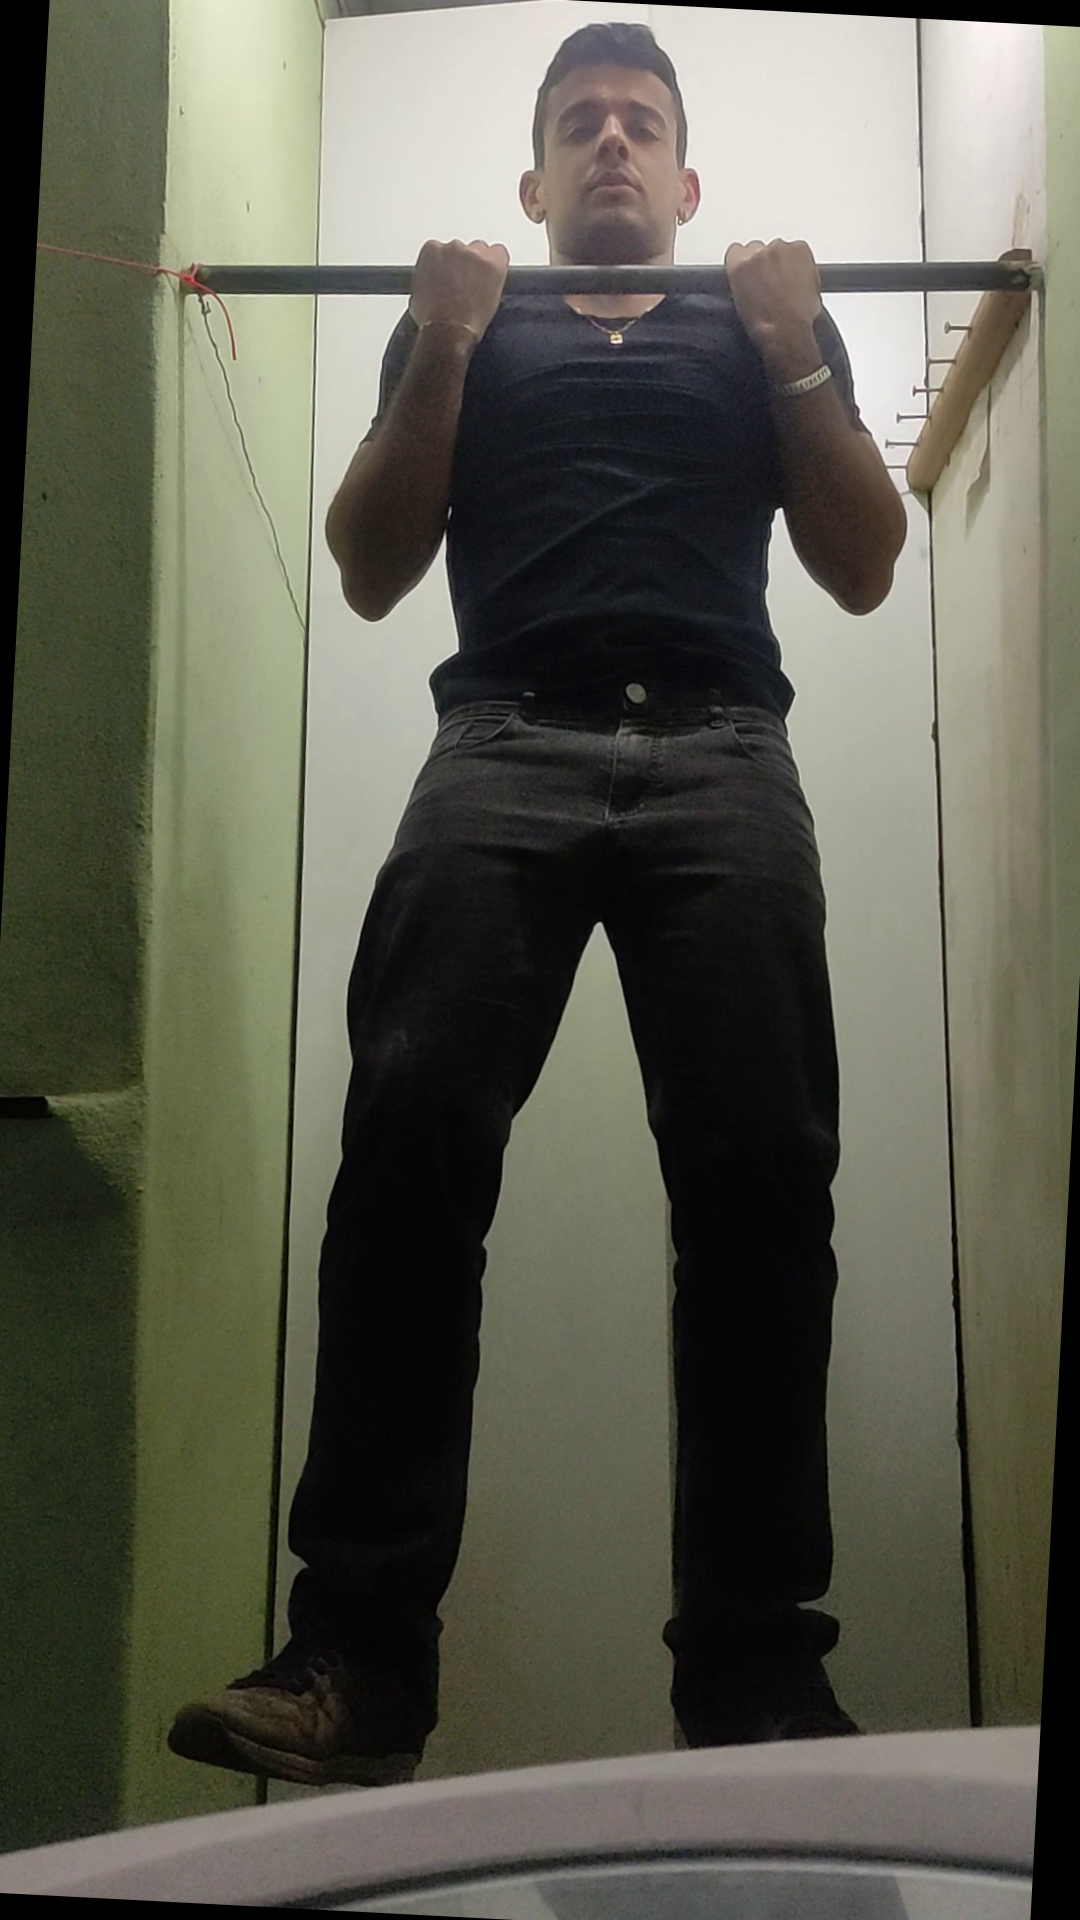
\includegraphics[scale=0.1]{img/desenvolvimento/ultrapassagemBarra/original.png}
        \caption*{Fonte - Próprio Autor.}
    \end{figure}
\end{frame}


\begin{frame}{Ultrapassagem do queixo à barra - Máscara cor da pele}
    \begin{figure}[!ht]
        \centering
            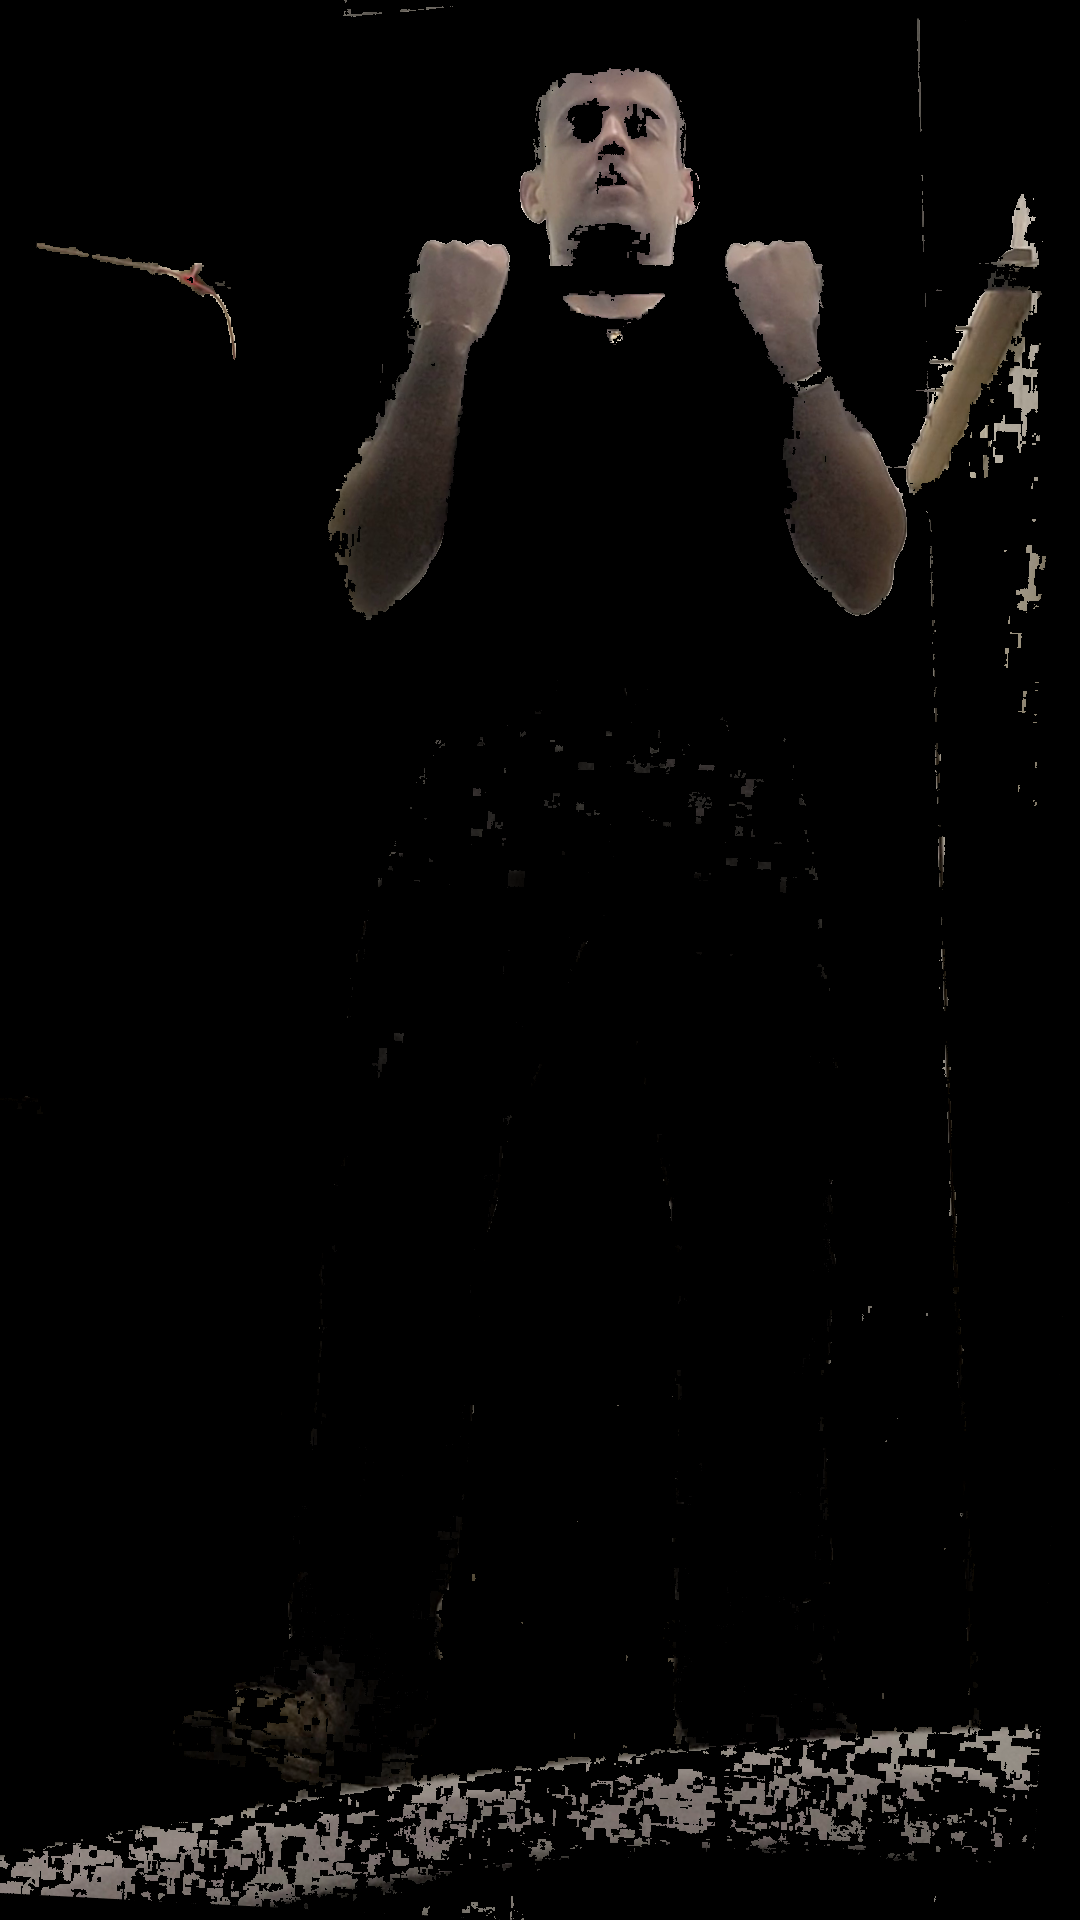
\includegraphics[scale=0.1]{img/desenvolvimento/ultrapassagemBarra/skin.png}
        \caption*{Fonte - Próprio Autor.}
    \end{figure}
\end{frame}

\begin{frame}{Ultrapassagem do queixo à barra - Escala de cinza}
    \begin{figure}[!ht]
        \centering
            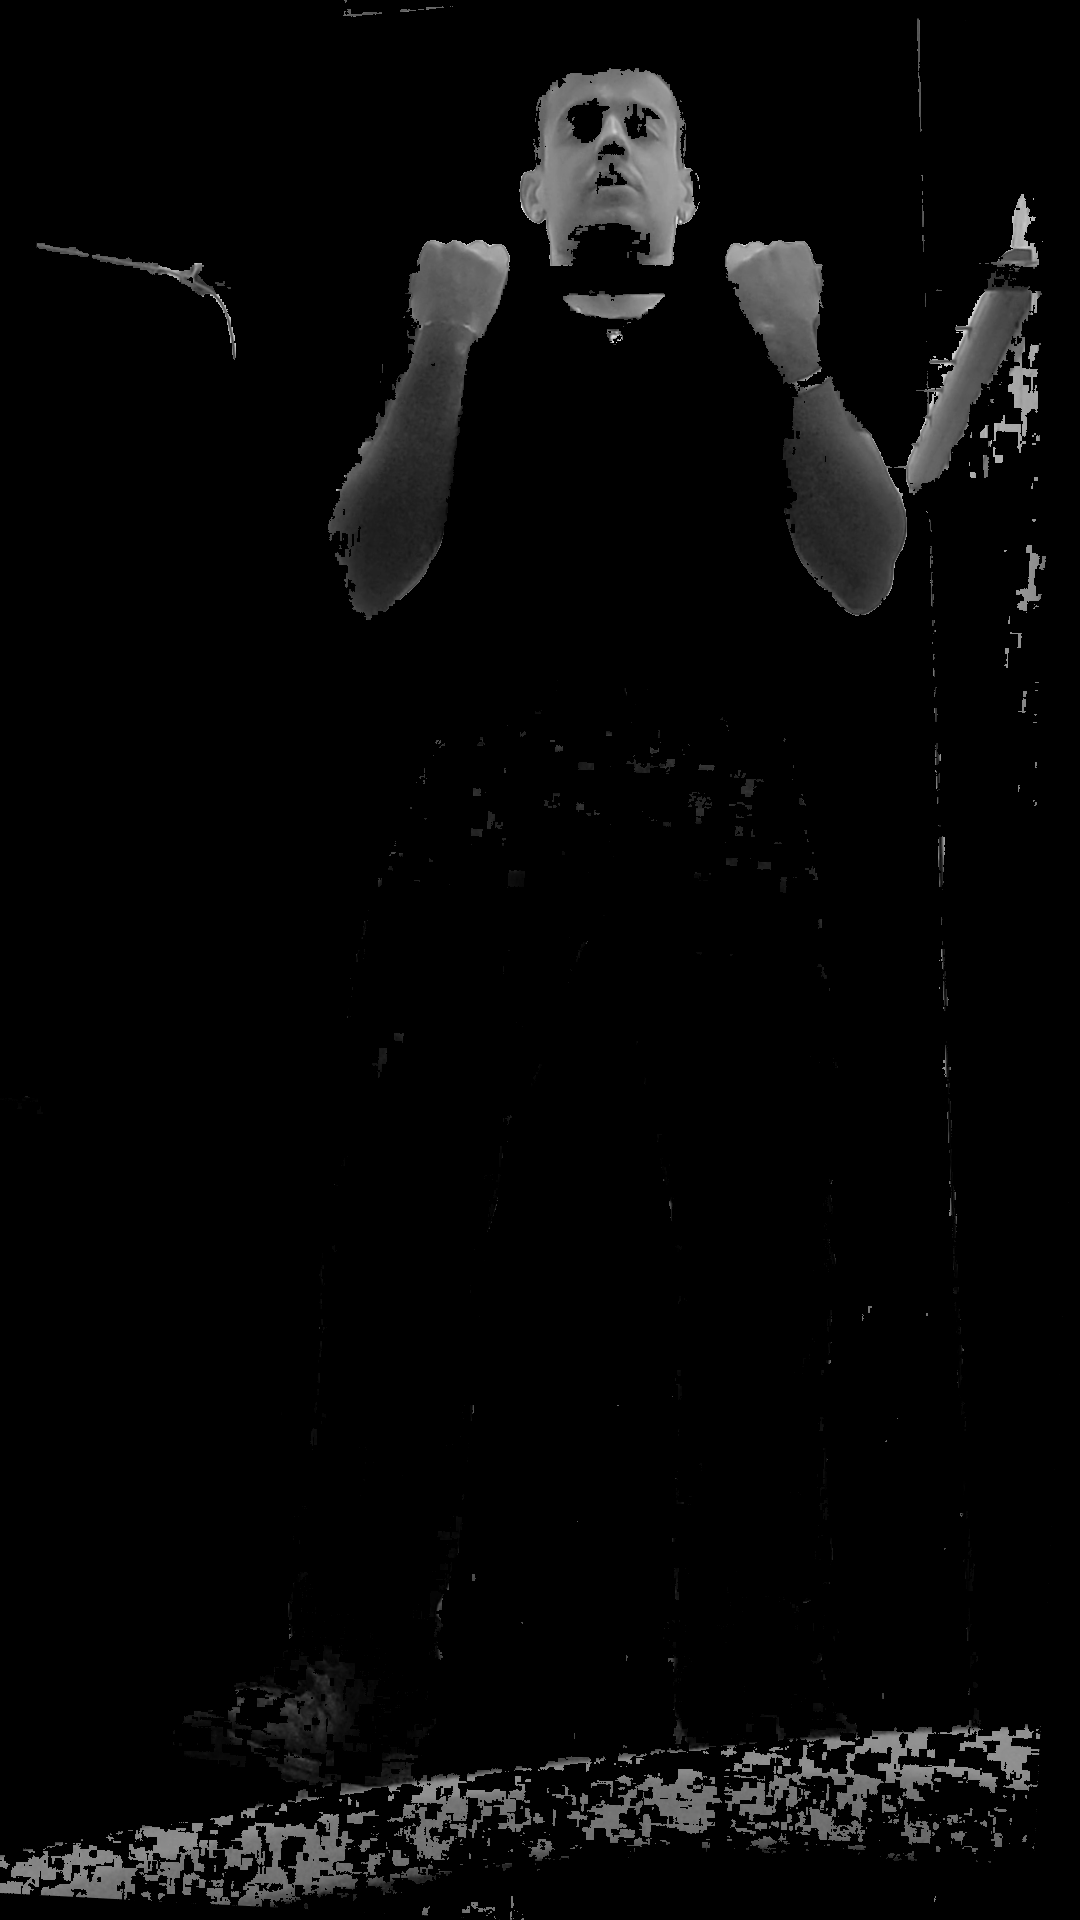
\includegraphics[scale=0.1]{img/desenvolvimento/ultrapassagemBarra/gray.png}
        \caption*{Fonte - Próprio Autor.}
    \end{figure}
\end{frame}

\begin{frame}{Ultrapassagem do queixo à barra - Limiarização}
    \begin{figure}[!ht]
        \centering
            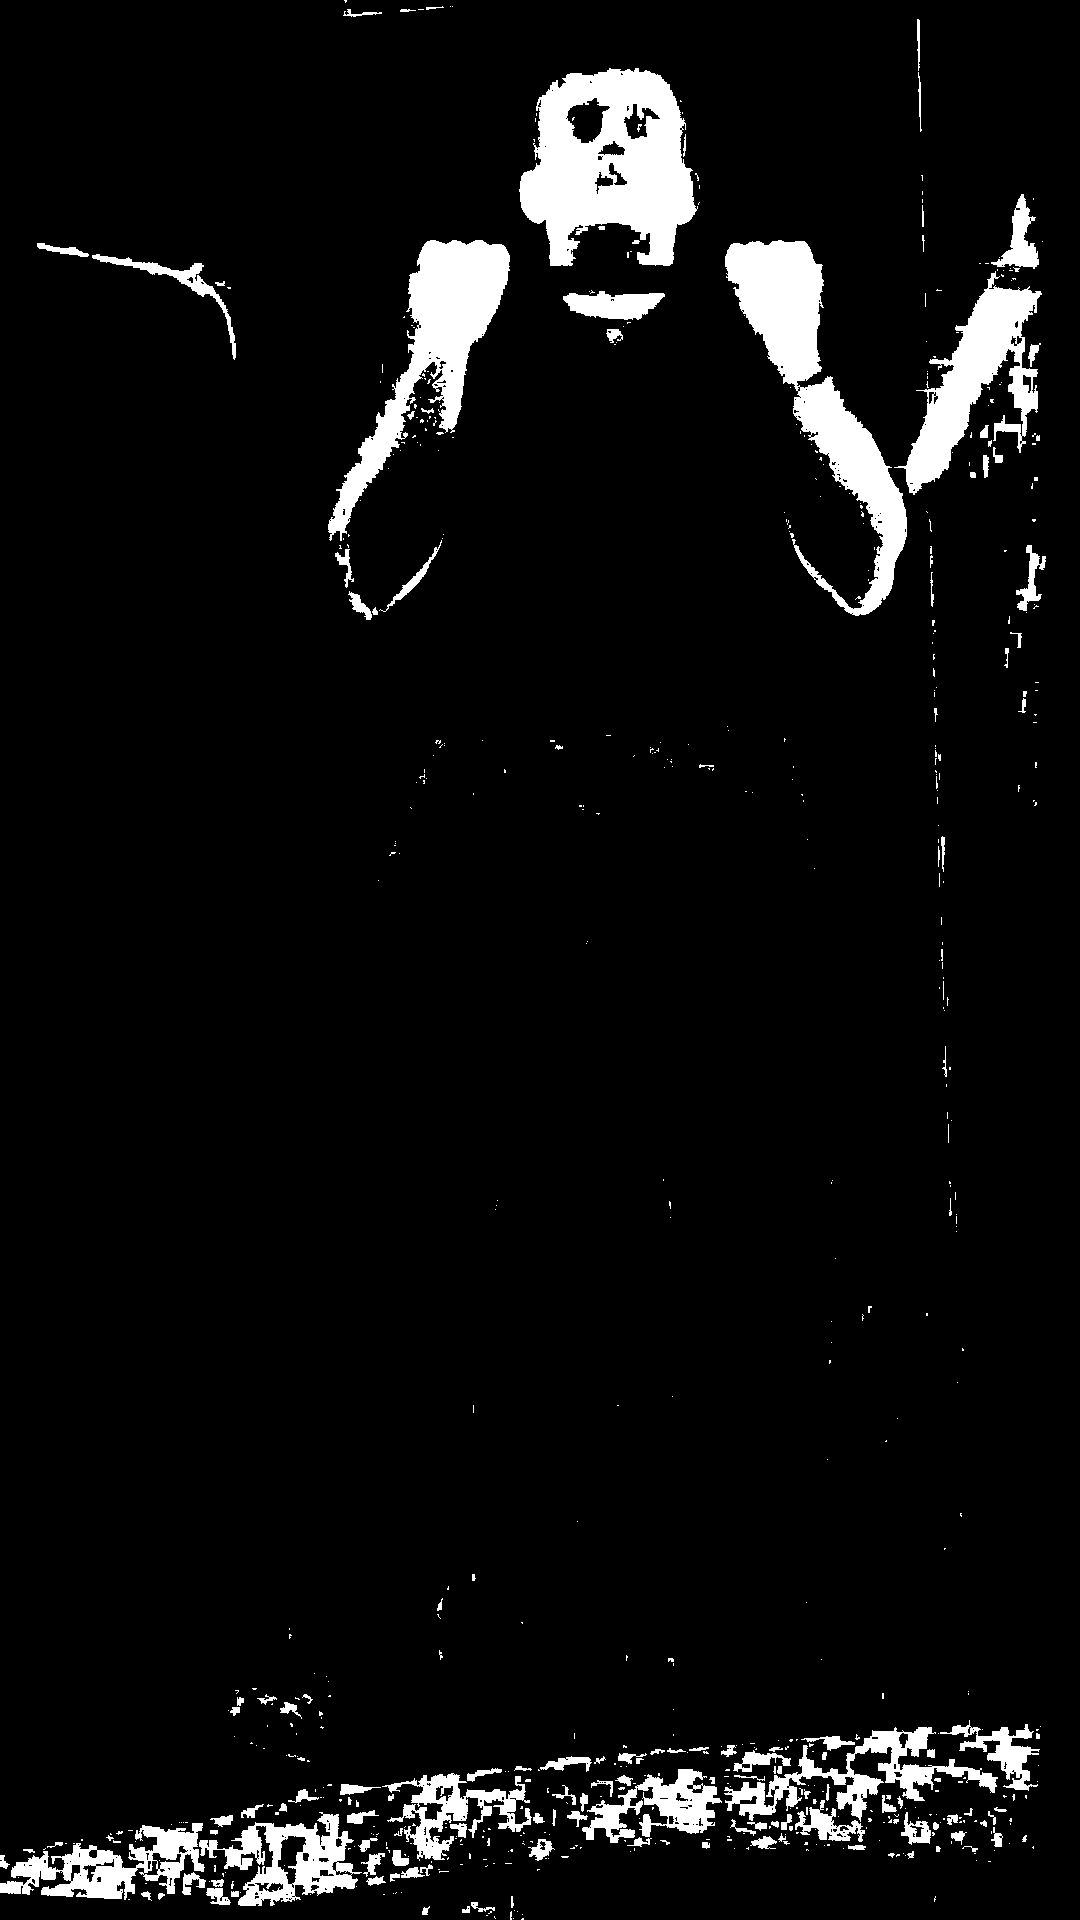
\includegraphics[scale=0.1]{img/desenvolvimento/ultrapassagemBarra/limited.png}
        \caption*{Fonte - Próprio Autor.}
    \end{figure}
\end{frame}


\begin{frame}{Ultrapassagem do queixo à barra - Máscara}
    \begin{figure}[!ht]
        \centering
            
\includegraphics[scale=0.1]{img/desenvolvimento/ultrapassagemBarra/mask_head.png}
        \caption*{Fonte - Próprio Autor.}
    \end{figure}
\end{frame}


\begin{frame}{Ultrapassagem do queixo à barra - Representação da área de interesse}
    \begin{figure}[!ht]
        \centering
            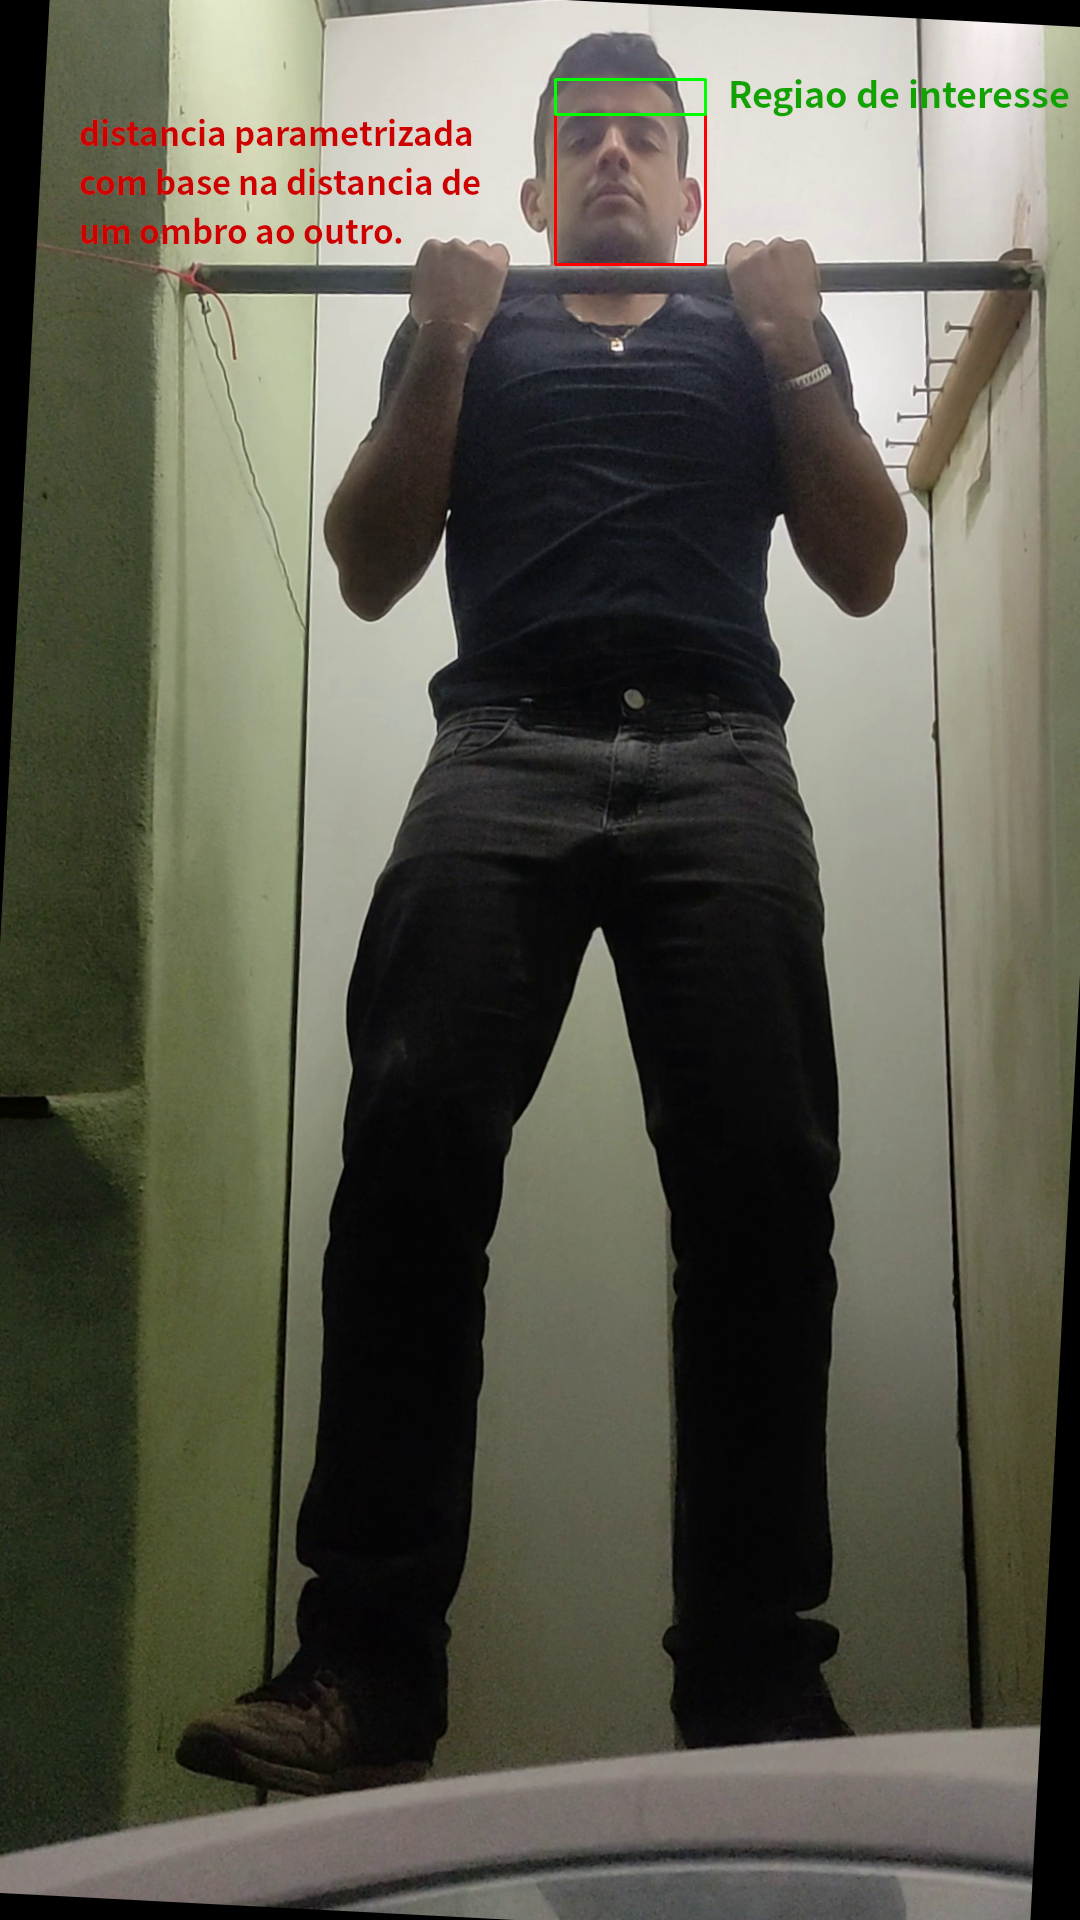
\includegraphics[scale=0.1]{img/desenvolvimento/ultrapassagemBarra/representação.png}
        \caption*{Fonte - Próprio Autor.}
    \end{figure}
\end{frame}


\begin{frame}{Ultrapassagem do queixo à barra - Imagem Segmentada}
    \begin{figure}[!ht]
        \centering
            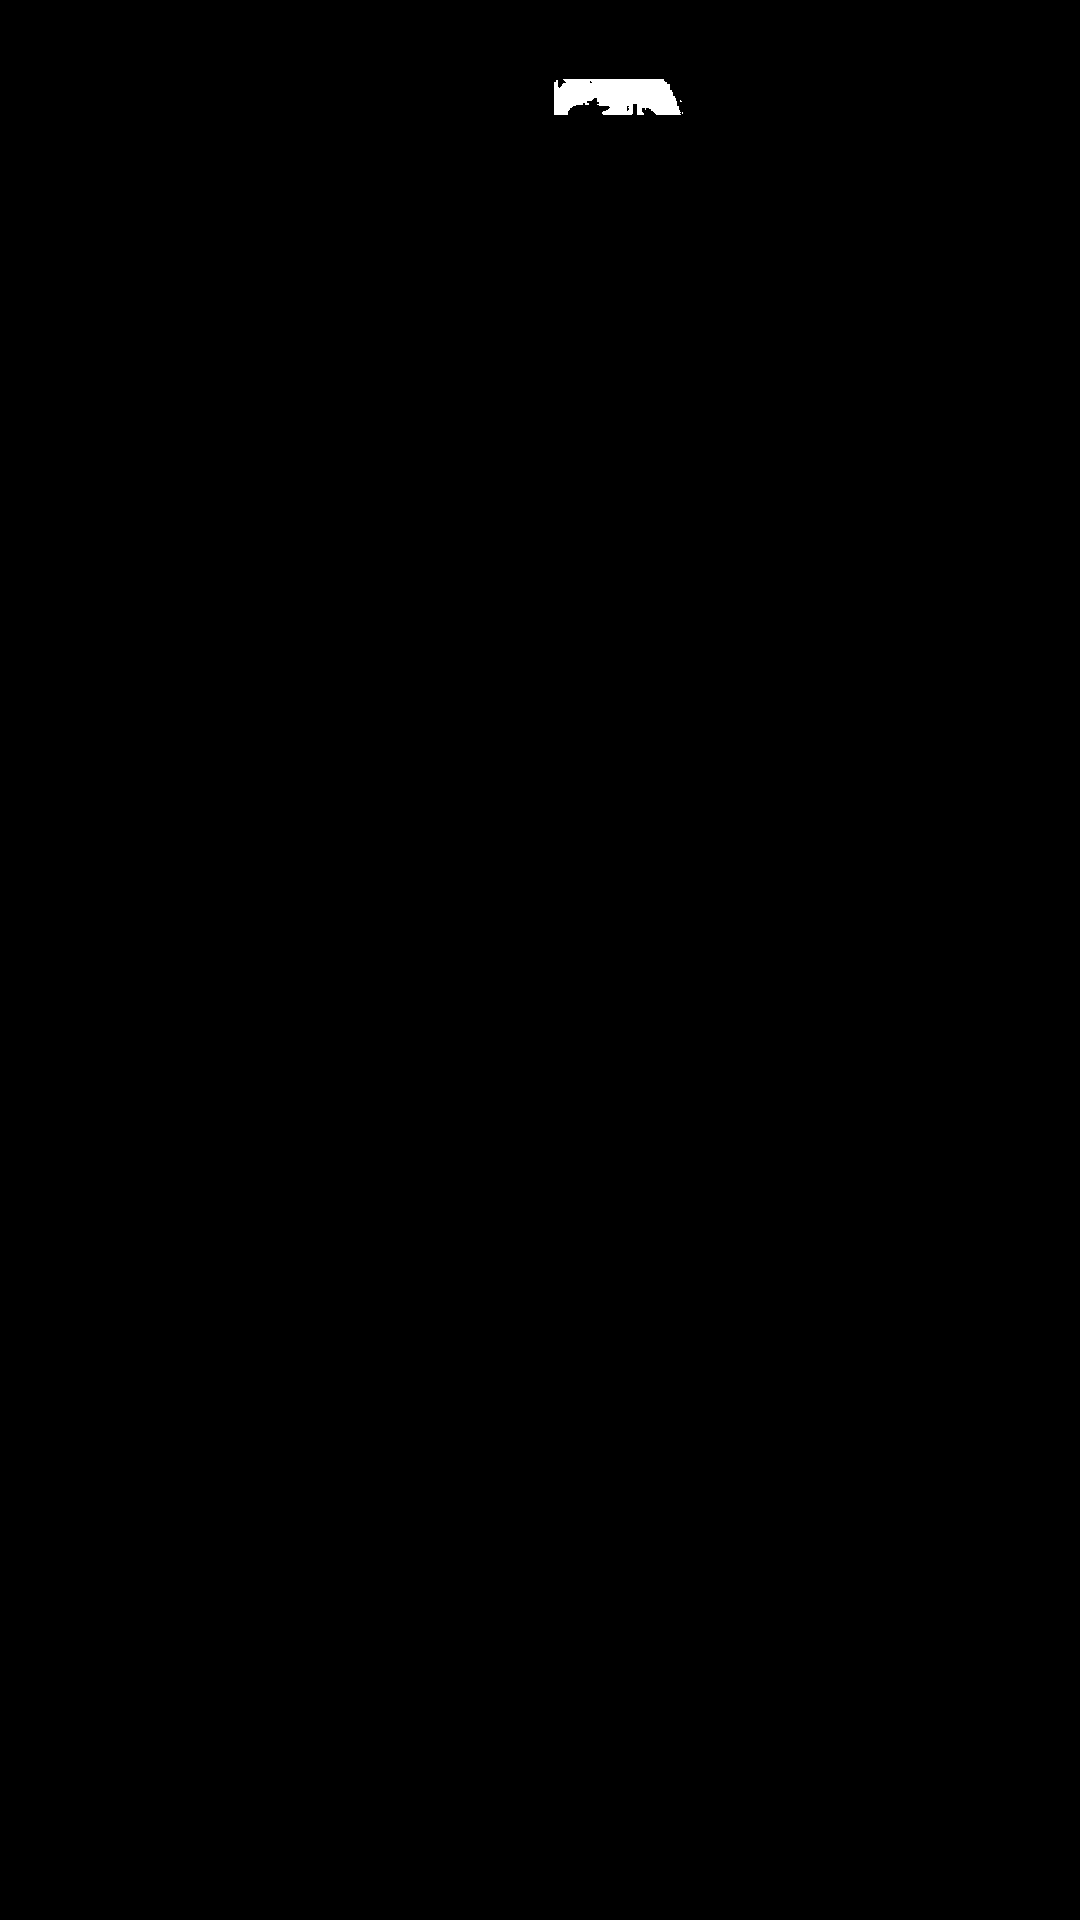
\includegraphics[scale=0.1]{img/desenvolvimento/ultrapassagemBarra/only_interesse.png}
        \caption*{Fonte - Próprio Autor.}
    \end{figure}
\end{frame}

%%%%%%%%%%%%%%%%%%%%%%%%%%%%%%%%%%%%%%%%%%%%%%%%%%%%%%%%%%%%%%%%%%%%
%%
%%                     Movimentação do quadril
%%
%%%%%%%%%%%%%%%%%%%%%%%%%%%%%%%%%%%%%%%%%%%%%%%%%%%%%%%%%%%%%%%%%%%%

\begin{frame}{Movimentação do quadril}

\begin{itemize}
        \item O movimento do quadril foi examinado de maneira semelhante à flexão e extensão
do cotovelo, no entanto, os pontos de referência utilizados foram o quadril, o joelho e o
tornozelo. 

        \item  A coxa foi considerada como o segmento de linha que se estende do quadril ao
joelho, enquanto a perna foi definida como o segmento de linha que se estende do joelho
até o tornozelo. Para avaliar a movimentação dos membros inferiores, foi analisado se o
ângulo entre os membros ou direito ou esquerdo excedia 15 graus de movimento.
    \end{itemize}
    
    
   

    
\end{frame}


\section{Resultados}
%%%%%%%%%%%%%%%%%%%%%%%%%%%%%%%%%%%%%%%%%%%%%%%%%%%%%%%%%%%%%%%%%%%%
%%
%%                     Resultados
%%
%%%%%%%%%%%%%%%%%%%%%%%%%%%%%%%%%%%%%%%%%%%%%%%%%%%%%%%%%%%%%%%%%%%%

\begin{frame}{Deteção da barra}
   \begin{figure}[H]
    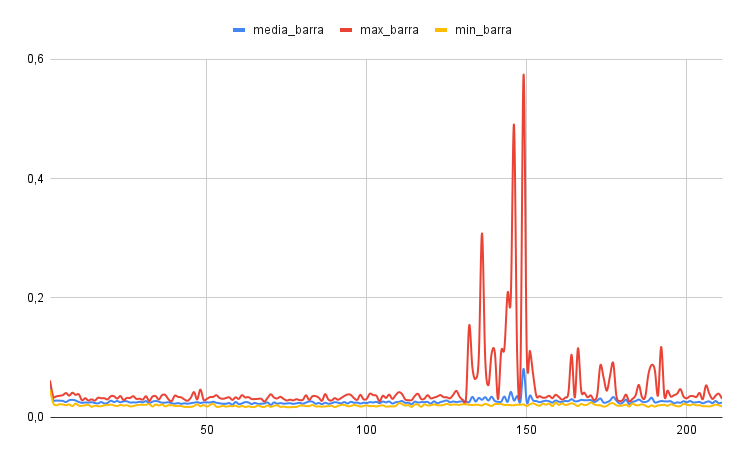
\includegraphics[width=11cm]{img/resultados/barra.png}
    {Fonte: Próprio Autor}
    \label{figura:configs_server}
    \end{figure}
\end{frame}

\begin{frame}{Inclinação da barra}
   \begin{figure}[H]
    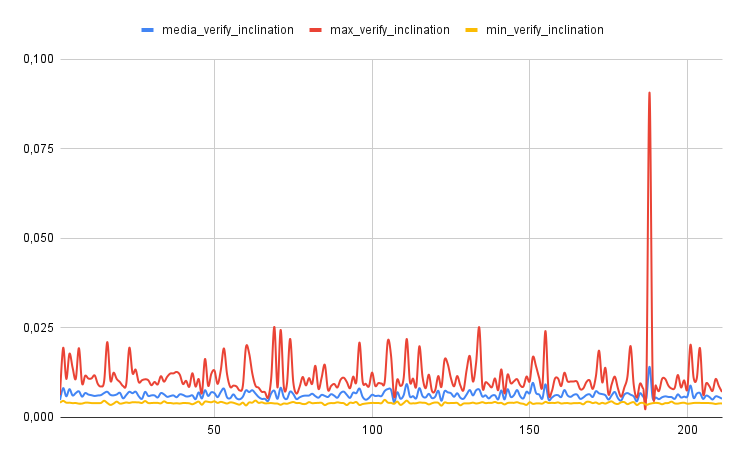
\includegraphics[width=11cm]{img/resultados/inclination.png}
    {Fonte: Próprio Autor}
    \label{figura:configs_server}
    \end{figure}
\end{frame}

\begin{frame}{Estimativa de pose humana}
   \begin{figure}[H]
    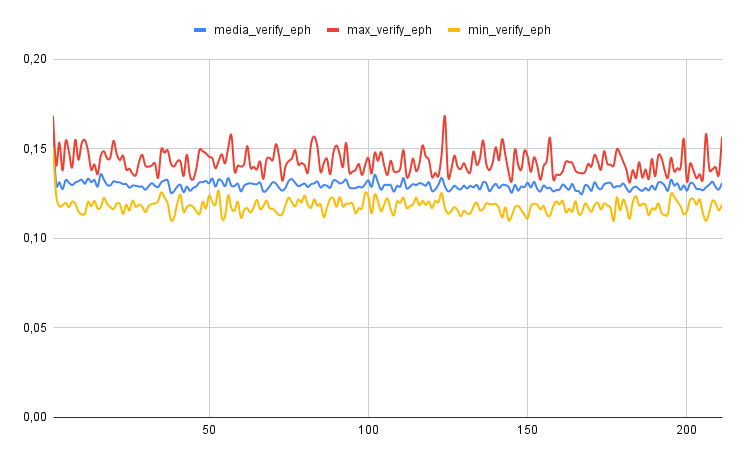
\includegraphics[width=11cm]{img/resultados/eph.png}
    {Fonte: Próprio Autor}
    \label{figura:configs_server}
    \end{figure}
\end{frame}

\begin{frame}{Construção do caracter do AFD}
   \begin{figure}[H]
    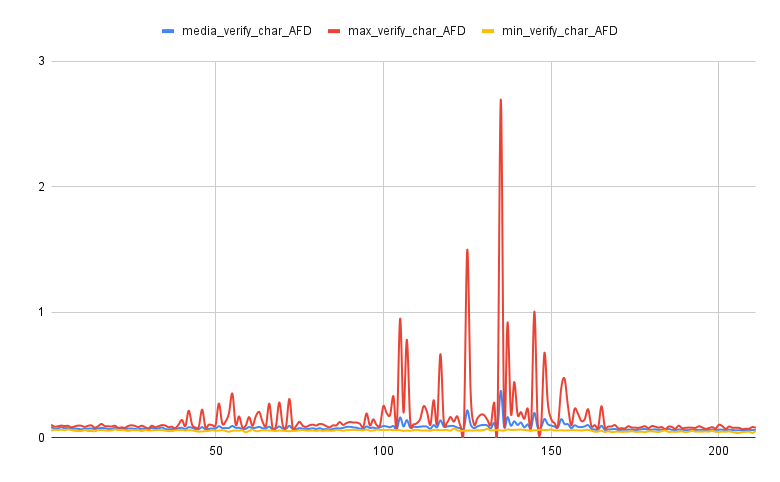
\includegraphics[width=11cm]{img/resultados/char_AFD.png}
    {Fonte: Próprio Autor}
    \label{figura:configs_server}
    \end{figure}
\end{frame}

\begin{frame}{Composição das funções que formam o caracter }
   \begin{figure}[H]
    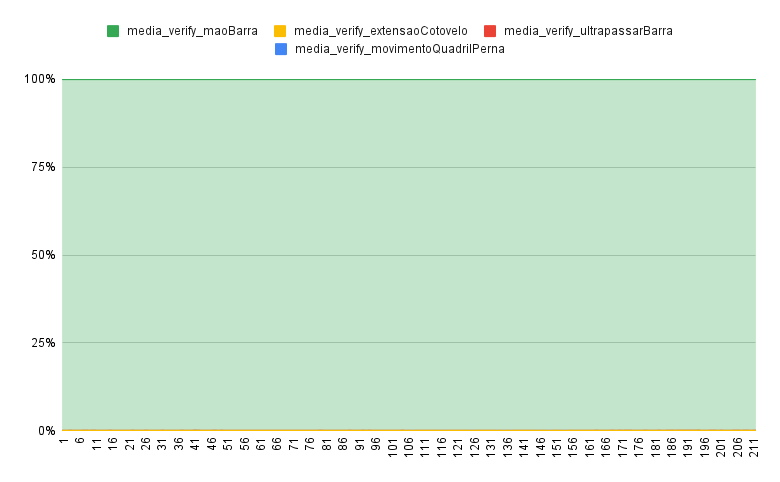
\includegraphics[width=11cm]{img/resultados/comp_char_AFD.png}
    {Fonte: Próprio Autor}
    \label{figura:configs_server}
    \end{figure}
\end{frame}

\begin{frame}{Mão na barra}
   \begin{figure}[H]
    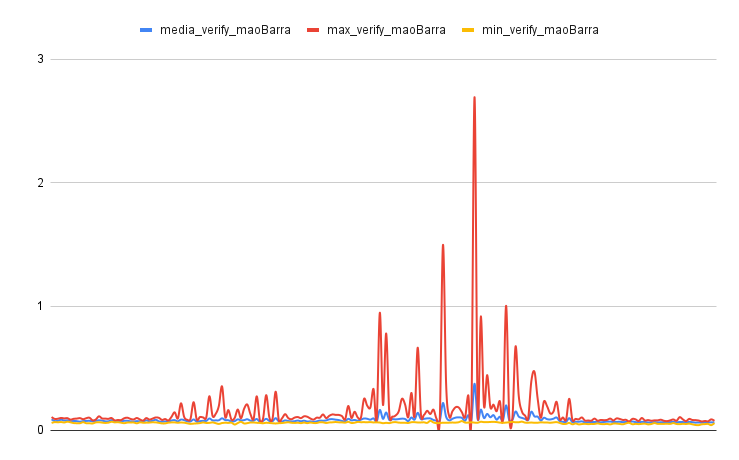
\includegraphics[width=11cm]{img/resultados/maoBarra.png}
    {Fonte: Próprio Autor}
    \label{figura:configs_server}
    \end{figure}
\end{frame}

\begin{frame}{Braço extendido}
   \begin{figure}[H]
    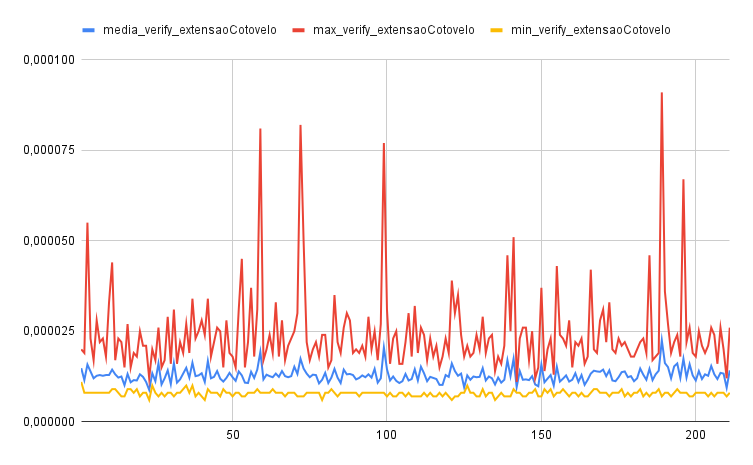
\includegraphics[width=11cm]{img/resultados/extensaoCotovelo.png}
    {Fonte: Próprio Autor}
    \label{figura:configs_server}
    \end{figure}
\end{frame}

\begin{frame}{Ultrapassar o queixo á barra}
   \begin{figure}[H]
    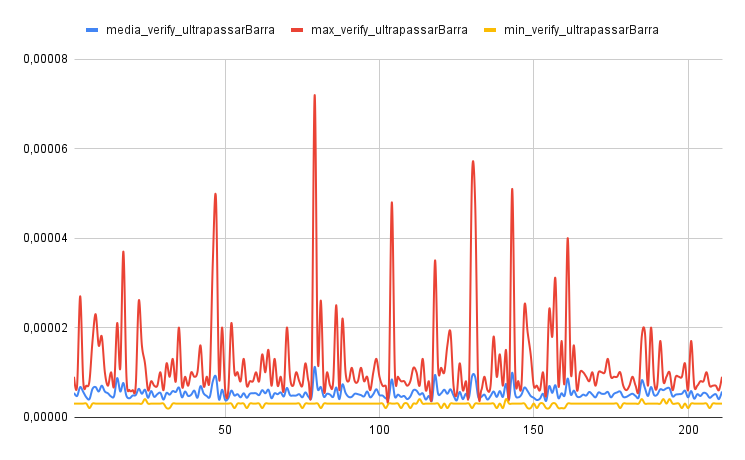
\includegraphics[width=11cm]{img/resultados/ultrapassarBarra.png}
    {Fonte: Próprio Autor}
    \label{figura:configs_server}
    \end{figure}
\end{frame}

\begin{frame}{Movimento das pernas e do quadril}
   \begin{figure}[H]
    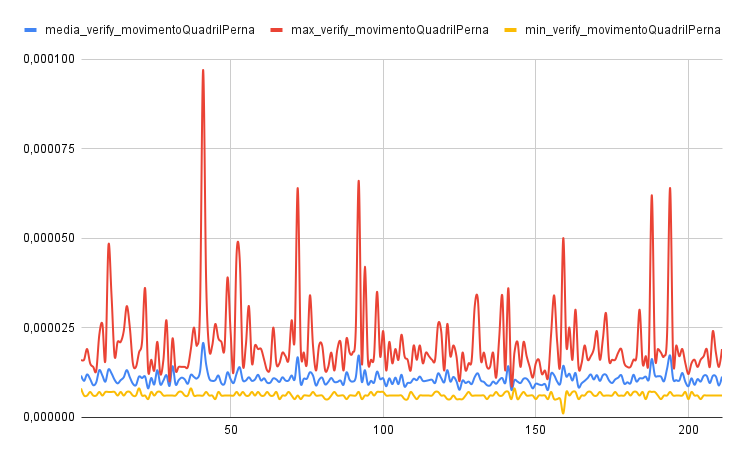
\includegraphics[width=11cm]{img/resultados/movimentoQuadril.png}
    {Fonte: Próprio Autor}
    \label{figura:configs_server}
    \end{figure}
\end{frame}




\begin{frame}{Processamento de um frame}
   \begin{figure}[H]
    \includegraphics[width=11cm]{img/resultados/process_cell.png}
    {Fonte: Próprio Autor}
    \label{figura:configs_server}
    \end{figure}
\end{frame}


\begin{frame}{Composição das funções necessárias para processar um frame}
   \begin{figure}[H]
    \includegraphics[width=11cm]{img/resultados/comp_process_cell_2.png}
    {Fonte: Próprio Autor}
    \label{figura:configs_server}
    \end{figure}
\end{frame}


\begin{frame}{Composição das funções necessárias para processar um frame}
   \begin{figure}[H]
    \includegraphics[width=11cm]{img/resultados/comp_process_cell_1.png}
    {Fonte: Próprio Autor}
    \label{figura:configs_server}
    \end{figure}
\end{frame}


%%%%%%%%%%%%%%%%%%%%%%%%%%%%%%%%%%%%%%%%%%%%%%%%%%%%%%%%%%%%%%%%%%%%
%%
%%                     Mensuração
%%
%%%%%%%%%%%%%%%%%%%%%%%%%%%%%%%%%%%%%%%%%%%%%%%%%%%%%%%%%%%%%%%%%%%%



\begin{frame}{Resultados Experimentos}
    \fontsize{7pt}{8pt}\selectfont
    \begin{table}[H]
    \centering
    \begin{tabular}{@{}cccccc@{}}
    \toprule
    \multicolumn{6}{c}{Tempos médios e menores tempos registrados para cada função}
    \\ \midrule
    Função & Tempo médio (s) & Menor tempo(s) \\
    \midrule
    barra & 0,03422 & 0,016335 \\
    verify\_inclination & 0,00603 & 0,00317 \\
    verify\_eph & 0,1293617 & 0,109623 \\
    verify\_angle\_member & 0,00013 & 0,000045 \\
    verify\_char\_AFD & 0,0753571 & 0,039386 \\
    verify\_AFD & 0,0000427 & 0,000016 \\
    \bottomrule
    \end{tabular}
    \label{tab:tempos_funcoes}
    \\
    {Fonte: Próprio Autor}
    \end{table}
\end{frame}






\begin{frame}{Resultados Experimentos}
    \fontsize{7pt}{8pt}\selectfont
    \begin{table}[H]
    \centering
    \begin{tabular}{@{}cccccc@{}}
    \toprule
    \\ \midrule
    Função & Tempo médio (s) & Menor tempo (s) \\
    \midrule
    verify\_maoBarra & 0,0747025 & 0,03924 \\
    verify\_extensaoCotovelo & 0,0000126 & 0,000006  \\
    verify\_ultrapassarBarra & 0,0000051 & 0,000002  \\
    verify\_movimentoQuadrilPerna & 0,0000104 & 0,000001  \\
    \bottomrule
    \end{tabular}
    \label{tab:tempos_funcoes_especificas}
    \\
    {Fonte: Próprio Autor}
    \end{table}
\end{frame}


\section{Considerações Finais}
\begin{frame}{Considerações Finais}
    \begin{itemize}
        \item O protótipo apresentado demonstrou uma \textbf{precisão satisfatória} na avaliação do movimento de barra fixa.
    
        \item \textbf{Dificuldade para a verificação do tipo de pegada} (pronada) devido a uma \textbf{imprecisão da ferramenta} em relação a detecção dos pontos de referência 17, 18 , 19 e 20
    
        \item O tempo médio de processamento de um frame foi de 0,2481895403 segundos. No entanto, para o processamento em tempo real de um vídeo com uma taxa de 24 frames por segundo, o tempo limite de processamento é de 0,0416 segundos por frame ou seja gastou\textbf{ 5,96 vezes mais tempo do que o esperado.}
    
        \item As 2 funções mais relevantes para a alta taxa de latência do processamento do frame são \textbf{’verify\_eph’} e \textbf{’verify\_maoBarra’} sendo responsável por cerca de \textbf{85.14\%} do tempo gasto por ’process\_cell’
    
        \item O protótipo produzido tem potencial para crescer e amadurecer;
    \end{itemize}
\end{frame}

\begin{frame}{Trabalhos Futuros}
    \begin{itemize}
        \item Melhoria dos pontos citados ( Execução e pegada pronada)
        \item Desejavel para trabalhos futuros um aprimoramento do relatório de modo que contabilize a quantidade de tempo gasto em cada tipo de contração muscular
        \item Elaborar estratégias para avançar com o grau de maturidade da ferramenta.
    \end{itemize}
\end{frame}


%%%%%%%% agradecimentos %%%%%%%%
%------------------------------------------------

%------------------------------------------------
%------------------------------------------------
%%%%%%%% referencias %%%%%%%%
\nocite{*}
\begin{frame}[allowframebreaks]{Referências}
\bibliographystyle{unsrt}
\bibliography{ref.bib}
\end{frame}

%%%%%%%% repete primeiro slide %%%%%%%%
\begin{frame}
\titlepage 
\end{frame}
\end{document}